\documentclass[9pt,xcolor={usenames, dvipsnames}]{beamer}
\usepackage{mathpazo} % Palatino for text only
\usepackage{amsmath}  % Standard math font remains Computer Modern
\usepackage{palatino}  % Sets both text and math to Times
% Explicitly ensure Palatino for text
\renewcommand{\rmdefault}{ppl}
\linespread{1.5}\selectfont
\mode<article>
{
  \usepackage{fullpage}
  \usepackage{epstopdf}
  \usepackage{pgf}
  \usepackage{hyperref}
  \usepackage{tikz}
  \usetikzlibrary{shapes.geometric, arrows, positioning}
  \setjobnamebeamerversion{example.beamer}
}
\usepackage{pdfpages}
\usepackage{comment}
% Theme and color settings
\mode<presentation>
{
   \usetheme{metropolis} % Metropolis theme with progress bars
   \usecolortheme{lily}
   \setbeamercovered{transparent}
}
\usepackage{pgfplots}
\pgfplotsset{compat=newest}
\usetikzlibrary{pgfplots.groupplots}
\usetikzlibrary{positioning}


% Standard math support
\usepackage{amsmath} 
\usepackage{bm}
\usepackage{graphicx}
\usepackage{pdflscape}
\usepackage{array}
\usepackage{tikz}
\usepackage{amssymb}
\usepackage[super]{natbib} 
\usepackage{pdfpages}
\usepackage{caption}
\usepackage{hyperref}
\usepackage{multicol}
\usepackage{booktabs}
\usepackage{mathtools}
\usepackage{blkarray}
\usepackage{colortbl}
\usepackage{listings}
\lstset{
    basicstyle=\ttfamily\footnotesize,
    breaklines=true,
    frame=single,
    numbers=left,
    numberstyle=\tiny,
    tabsize=2
}
\definecolor{applegreen}{rgb}{0, 0.5, 0.0}
\definecolor{darkorange}{rgb}{0.8, 0.40, 0.0}


\newcommand{\backupbegin}{
   \newcounter{finalframe}
   \setcounter{finalframe}{\value{framenumber}}
}
\newcommand{\backupend}{
   \setcounter{framenumber}{\value{finalframe}}
}

\usepackage{amssymb, amsmath, amsthm}
\usepackage{tcolorbox} % For fancy boxes

% Define theorem styles
\theoremstyle{definition}
\newtheorem{proposition}{Proposition}

\usepackage{ulem}  % for strikethrough
\usepackage{tikz}
\usepackage{standalone}
\usetikzlibrary{arrows.meta, chains, positioning, shapes.geometric}

\usepackage[english]{babel}
\tikzset{
   invisible/.style={opacity=0,text opacity=0},
   visible on/.style={alt=#1{}{invisible}},
   alt/.code args={<#1>#2#3}{%
      \alt<#1>{\pgfkeysalso{#2}}{\pgfkeysalso{#3}} % \pgfkeysalso doesn't change the path
   },
}

\geometry{papersize={16cm, 9cm}}

\usepackage[english]{babel}
\tikzset{
  invisible/.style={opacity=0,text opacity=0},
  visible on/.style={alt=#1{}{invisible}},
  alt/.code args={<#1>#2#3}{%
    \alt<#1>{\pgfkeysalso{#2}}{\pgfkeysalso{#3}} % \pgfkeysalso doesn't change the path
  },
}

\usepackage{remreset}% tiny package containing just the \@removefromreset command
\makeatletter
\@removefromreset{subsection}{section}
\beamer@compresstrue
\makeatother

\definecolor{cadmiumgreen}{rgb}{0.0, 0.42, 0.24}

\mode<presentation>
\setbeamercovered{transparent}

\mode<all>
\useoutertheme[section=false]{miniframes}

\setbeamertemplate{navigation symbols}{}

% Hide the mini frame dots but keep section names
\setbeamertemplate{mini frame}{}
\setbeamertemplate{mini frame in current subsection}{}
\setbeamertemplate{mini frame in current section}{}

% Customize headline to show only section names
\makeatletter
\setbeamertemplate{headline}{%
    \vskip1ex% Adjust spacing above
    \ifnum\value{section}>0% Start after Introduction
    \hbox to \paperwidth{%
        \hfill%
        \begin{beamercolorbox}[ht=1.5ex,dp=0.75ex,leftskip=1mm,rightskip=1mm]{section in head/foot}%
            \usebeamerfont{section in head/foot}%
            \insertsectionnavigationhorizontal{0.9\paperwidth}{}{}% Section names only
        \end{beamercolorbox}%
        \hfill
    }%
    \fi
    \vskip1.5ex% Adjust spacing below
}
\makeatother

% Define custom colors
\definecolor{darkblue}{HTML}{1A2B49}       % Dark Blue for titles
\definecolor{red}{HTML}{C0392B}            % Red for frame titles
\definecolor{bluebullet}{HTML}{2980B9}     % Blue for bullets
\definecolor{darkgray}{HTML}{2E2E2E}       % Dark gray for body text
%— a "less-dark" red (≈ fire-brick) —
\definecolor{softred}{RGB}{178,34,34}   % (178, 34, 34)
\definecolor{softgreen}{RGB}{34,139,34}  % forest green

%— the green used in the figure —
\definecolor{graphgreen}{RGB}{0,128,0}  % pure #008000
% Define custom colors
\definecolor{firmboxcolor}{HTML}{2C3E50}  % Dark blue for firm boxes
\definecolor{firmtextcolor}{HTML}{1A2B49} % Dark blue for firm titles
\definecolor{lightgrayarrow}{HTML}{BDC3C7} % Light gray for arrows within firms
\newcounter{propCounter}
\setcounter{propCounter}{1}
\renewcommand{\thepropCounter}{\arabic{propCounter}}

% Define a fancy boxed proposition environment using the new counter
\newtcolorbox[auto counter, number within=propCounter]{propositionbox}[1][]{%
    colback=darkblue!5!white, colframe=darkblue,
    fonttitle=\bfseries, title=Proposition~\thepropCounter: #1}


% Customize slide titles (frameless, dark blue)
\setbeamercolor{frametitle}{fg=black}      % Title color outside the frame
\setbeamerfont{frametitle}{size=\LARGE,series=\bfseries}  % Large bold titles
% Set global button colors (optional)
\definecolor{lightgray}{RGB}{211, 211, 211}  % RGB values for light gray
\setbeamercolor*{button}{bg=lightgray, fg=darkblue}

% Remove title frame
\setbeamertemplate{frametitle}{%
  \vskip0.5em%
  \insertframetitle%
  \vskip0.5em%
}

% Customize bullets
\setbeamercolor{item}{fg=bluebullet}  % Blue bullets
\setbeamertemplate{itemize item}{\color{bluebullet}$\bullet$}  % Customize bullet appearance

% Body text color
\setbeamercolor{normal text}{fg=darkgray}  % Dark gray text

% Font settings (you can keep Metropolis default sans-serif)
\renewcommand{\familydefault}{\sfdefault}

% Customize title and author (adjusted size)
\setbeamerfont{title}{size=\Large,series=\bfseries}
\setbeamercolor{title}{fg=darkblue}

\setbeamerfont{author}{size=\large}
\setbeamercolor{author}{fg=darkblue}

\setbeamerfont{institute}{size=\normalsize, series=\itshape}
\setbeamercolor{institute}{fg=darkblue}

% Title, Author, and Institute Information
\title{\Large Functional Approximation with (Chebyshev) Polynomials}
\author[Bocconi University]{Piero De Dominicis}
\institute{Bocconi University \\ QuantEcon Reading Group}
\date{}  % No date displayed

\begin{document}

\frame{\maketitle}

\metroset{sectionpage=none}
\section{Introduction}

\begin{frame}{Overview}

    \begin{itemize}
        \item \textbf{\textcolor{darkblue}{Goal:}} Learn how to approximate functions using (Chebyshev) polynomials
        \item \textbf{\textcolor{darkblue}{Two Examples:}}
        \begin{enumerate}
            \item \textbf{1D approximation}: Approximate $f(x) = \exp(x)$ on $[0,1]$
            \item \textbf{2D approximation}: Approximate $f(x,y) = \exp(x)\exp(y)$ on $[0,1] \times [-1,0]$
        \end{enumerate}
        \item \textbf{\textcolor{darkblue}{Motivation:}} Solve Equilibrium Model in Economics (Neoclassical Growth Model)
        \item \textbf{\textcolor{darkblue}{Challenge:}} When solving a model, we need to solve for an unknown function!
        \item \textbf{\textcolor{darkblue}{Solution:}} We use first-order and equilibrium conditions to find the unknown function 
    \end{itemize}
    
\end{frame}

\begin{frame}{The Neoclassical Growth Model: Problem Setup}

\visible<1->{
    \textbf{\textcolor{darkblue}{Household's Problem:}}
    \begin{align*}
    \max_{c \geq 0, \ell \in [0,1]} \quad & \log c - \chi \frac{\ell^{1+\frac{1}{\nu}}}{1+\frac{1}{\nu}} + \beta \mathbb{E}[V(a';z',K')] \\
    \text{subject to:} \quad & c + p(z,K) \leq w(z,K) \ell + (p(z,K) + \Pi(z,K))a
    \end{align*}
}

\visible<2->{
    \textbf{\textcolor{darkblue}{Firm's Problem:}}
    \begin{align*}
    J(k;z,K) = \max_{k' \geq 0, \pi, \ell \in [0,1]} \quad & \pi + \beta \mathbb{E}[\Lambda(S',S) J(k';z',K')] \\
    \text{subject to:} \quad & k' + w(z,K) \ell + \pi \leq y + (1-\delta)k \\
    & y = e^z k^{\alpha} \ell^{1-\alpha}
    \end{align*}
}

\end{frame}

\begin{frame}{Equilibrium Conditions}

\visible<1->{
    \textbf{\textcolor{darkblue}{First-Order Conditions:}}
    \begin{align*}
    \chi \ell(z,K)^{\frac{1}{\nu}} &= (1-\alpha) \frac{y(z,K)}{\ell(z,K)} \frac{1}{c(z,K)} \quad \text{(Intratemporal)} \\
    1 &= \mathbb{E}_S\left[\beta \frac{c(z,K)}{c(z',K')} \left(\alpha \frac{y(z',K')}{k(z',K')} + 1 - \delta\right)\right] \quad \text{(Euler)}
    \end{align*}
}

\visible<2->{
    \textbf{\textcolor{darkblue}{Resource Constraints:}}
    \begin{align*}
    y(z,K) &= c(z,K) + k(z,K) - (1-\delta)K \\
    y(z,K) &= e^z K^{\alpha} \ell(z,K)^{1-\alpha}
    \end{align*}
}

\end{frame}

\begin{frame}{Why Chebyshev Polynomials?}

\visible<1->{
    \textbf{\textcolor{darkblue}{Key Insight:}} Instead of solving for function values at infinitely many points, we approximate:
    \begin{equation*}
    c(z,K) \approx \sum_{i=0}^{n_z-1} \sum_{j=0}^{n_k-1} \gamma_{ij} T_i(\tilde{z}) T_j(\tilde{K})
    \end{equation*}
    where $T_i(\tilde{z})$, $T_j(\tilde{K})$ are Chebyshev polynomials evaluated at \textbf{Chebyshev nodes} $\tilde{z}, \tilde{K} \in [-1,1]$, and $\gamma_{ij}$ are \textbf{finitely many coefficients}
}

\visible<2->{
    \textbf{\textcolor{darkblue}{Advantages:}}
    \begin{itemize}
        \item \textbf{Fast convergence}: Few parameters needed for smooth functions
        \item \textbf{Optimal nodes}: Chebyshev nodes minimize maximum approximation error ("worst-case error")
        \item \textbf{Global approximation}: Can evaluate at any point, not just grid points
    \end{itemize}
}

\visible<3->{
    \textbf{\textcolor{softred}{Disadvantages:}}
    \begin{itemize}
        \item \textbf{Curse of dimensionality}: Computational cost grows exponentially with $\#$ of state variables
        \item \textbf{Requires smooth functions}: Poor performance for non-smooth or discontinuous functions
    \end{itemize}
}

\end{frame}

\begin{frame}{What are Chebyshev Polynomials?}

\visible<1->{
    \textbf{\textcolor{darkblue}{Definition:}} Chebyshev polynomials are a sequence of orthogonal polynomials defined on $[-1, 1]$
    
    \textbf{\textcolor{darkblue}{Recursive Definition:}} $T_0(x) = 1$; $T_1(x) = x$; $T_{n+1}(x) = 2x T_n(x) - T_{n-1}(x)$, $n \geq 1$
    
    where $x \in [-1,1]$ is a Chebyshev node (the input to the polynomial)

    \begin{center}
    \begin{figure}
        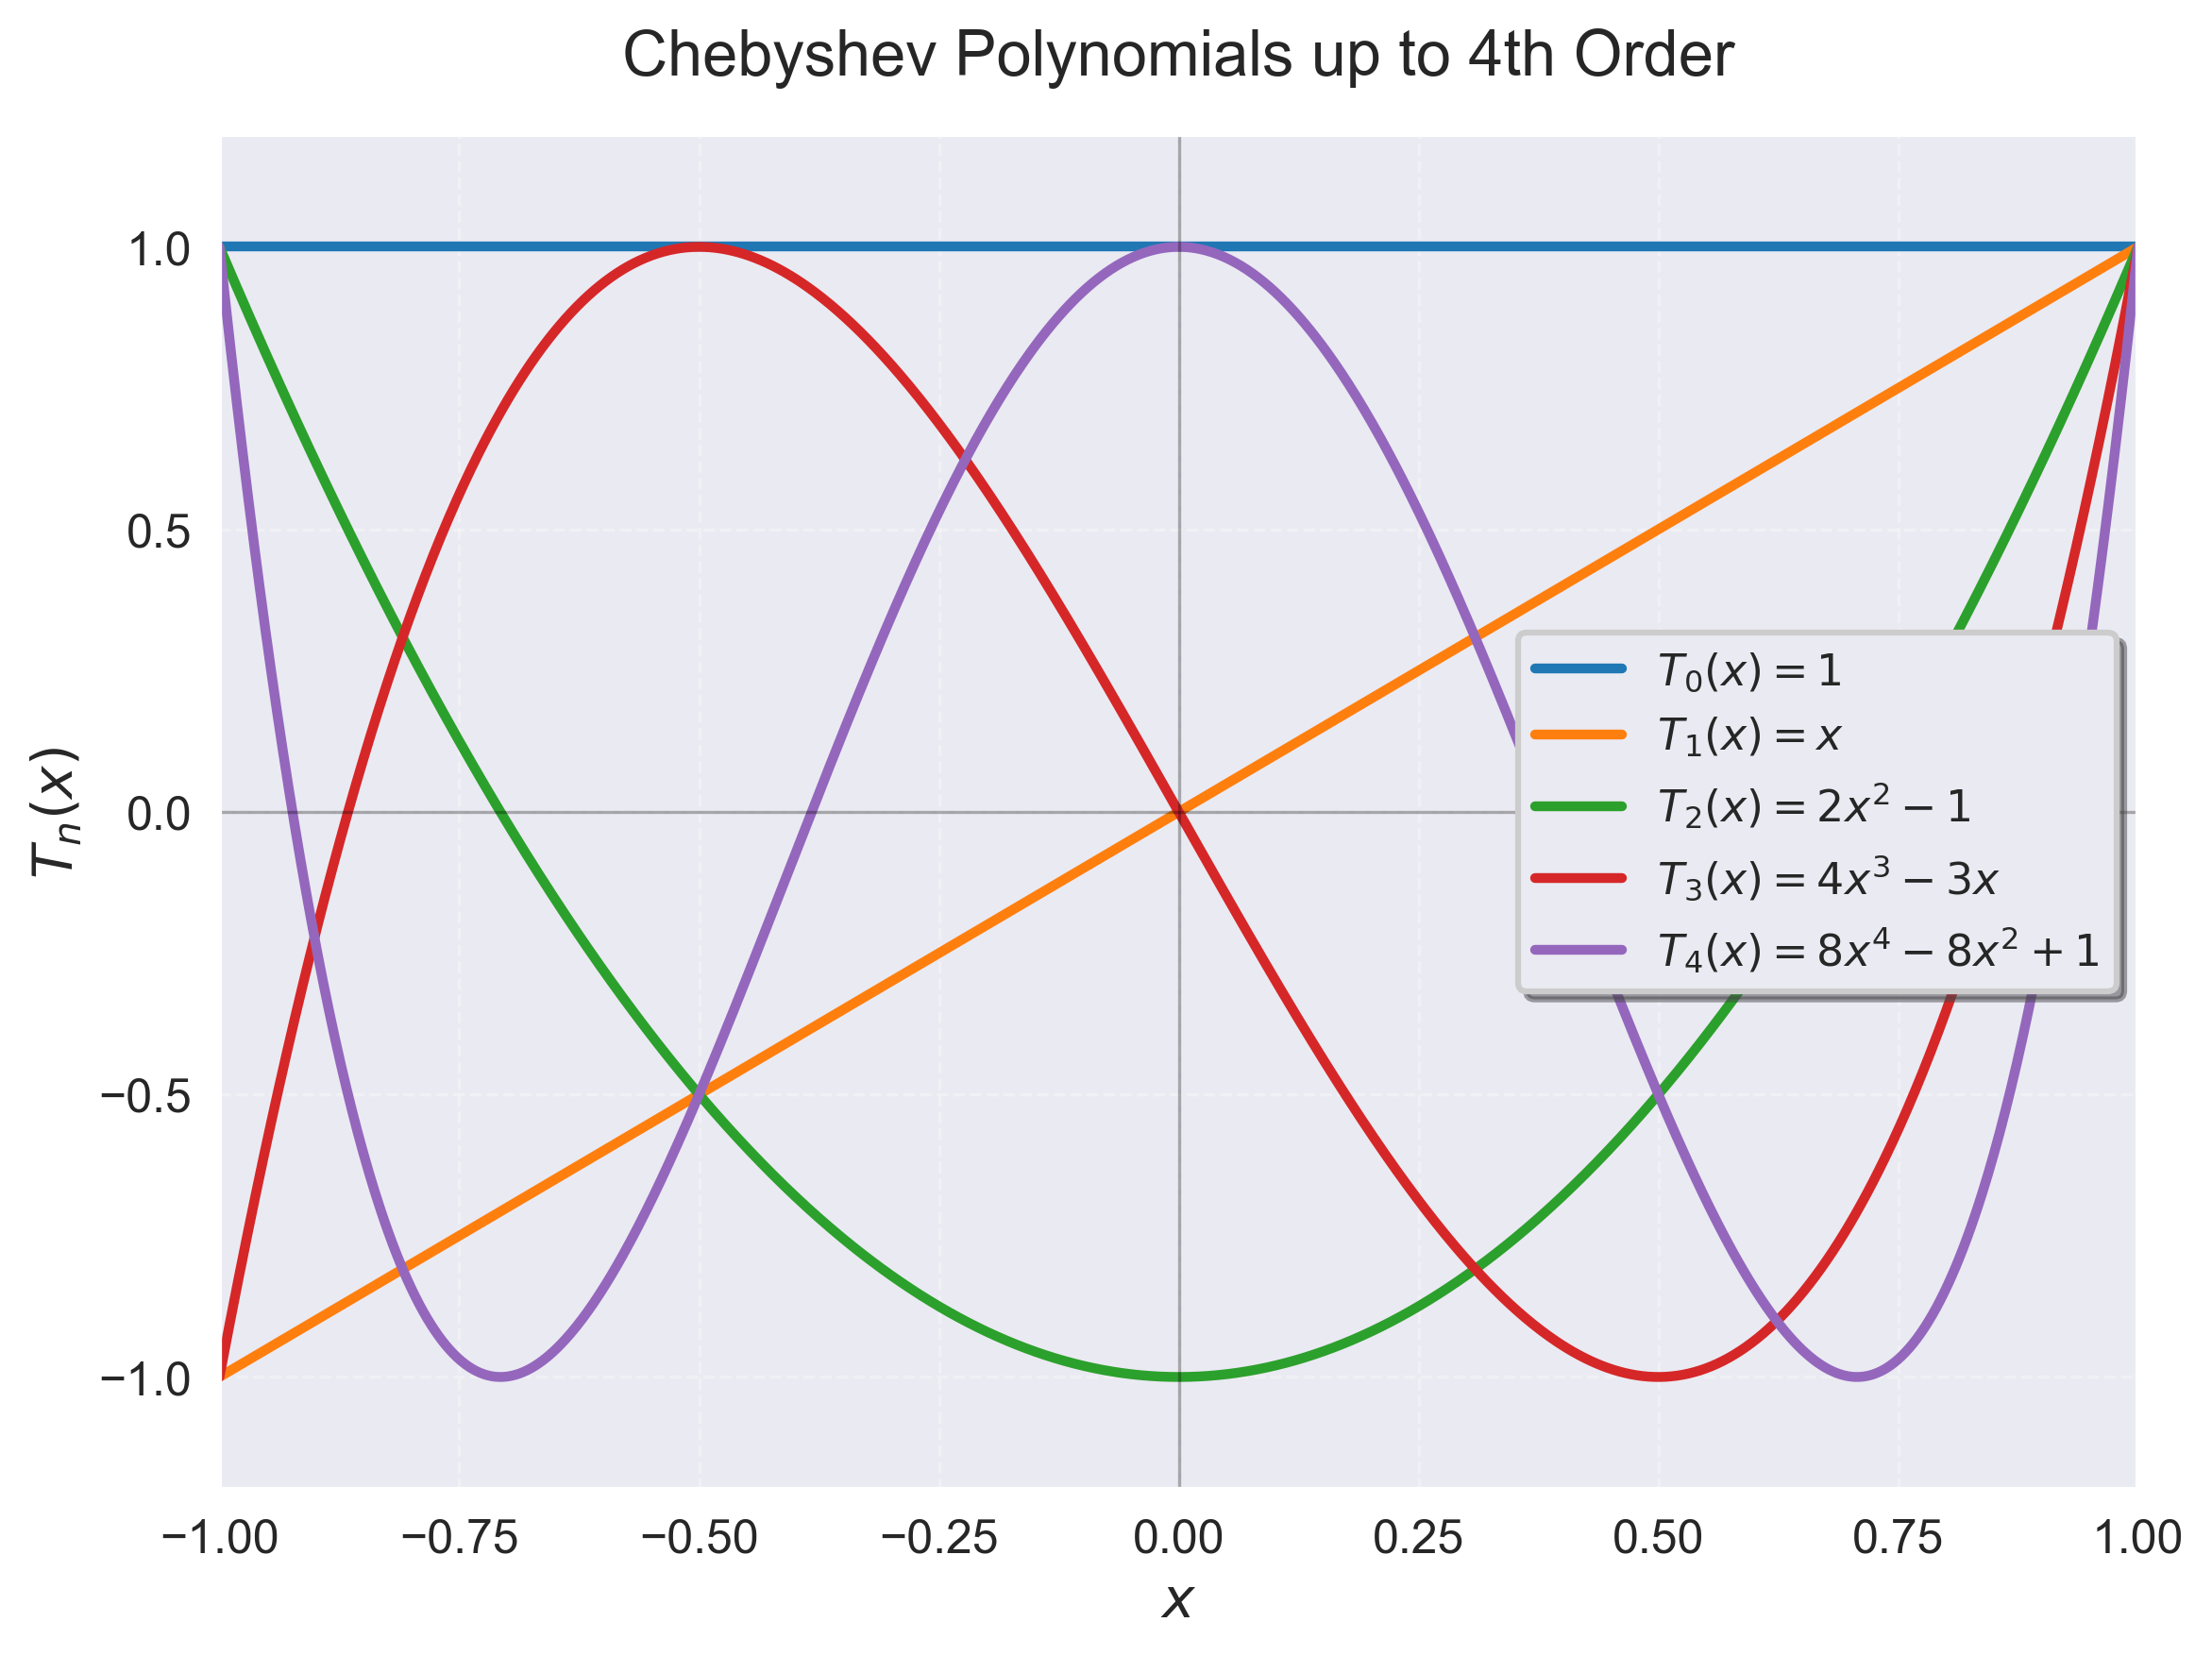
\includegraphics[width=0.5\textwidth]{figures/teaching/chebyshev_polynomials_4th_order.png}
    \end{figure}
    \end{center}
    
    \textbf{\textcolor{darkblue}{Key Properties:}}
    \begin{itemize}
        \item \textbf{Orthogonal:} $\int_{-1}^{1} \frac{T_i(x) T_j(x)}{\sqrt{1-x^2}} dx = 0$ for $i \neq j$
        \item \textbf{Bounded:} $|T_n(x)| \leq 1$ for all $x \in [-1,1]$
        \item \textbf{Optimal for approximation:} Minimize maximum error on $[-1,1]$
    \end{itemize}
}

\end{frame}

\begin{frame}{Outline}

\begin{enumerate}
    \item \textbf{Introduction}
        \vspace{0.2cm}
      
    \item \textbf{Example 1: Univariate Approximation (1D)}
        \begin{itemize}
            \item Step-by-step procedure
            \item Choice of grid and polynomial order
            \item Comparison with Taylor polynomials
        \end{itemize}
        \vspace{0.3cm}
      
    \item \textbf{Example 2: Bivariate Approximation (2D)}
        \begin{itemize}
            \item Step-by-step procedure
            \item Tensor product construction
            \item Optimization routine
        \end{itemize}
        \vspace{0.3cm}
        
    \item \textbf{Solving the Neoclassical Growth Model}
        \begin{itemize}
            \item Complete solution algorithm
            \item Application of techniques from examples
        \end{itemize}
        \vspace{0.3cm}
        
\end{enumerate}

\end{frame}

\setcounter{section}{2}
\section[Example 1: 1D Approximation]{Example 1: Univariate Approximation}

\begin{frame}{Example 1: Problem Setup}

\visible<1->{
    \textbf{\textcolor{darkblue}{Objective:}} Approximate the function
    \begin{equation*}
    f(x) = e^x
    \end{equation*}
    on the domain $x \in [-1, 1]$
}

\visible<2->{
    \textbf{\textcolor{darkblue}{Approximation Form:}}
    \begin{equation*}
    f(x) \approx \sum_{n=0}^{p_x-1} \gamma_n T_n(\tilde{x})
    \end{equation*}
    where $\tilde{x}$ is the Chebyshev domain $[-1,1]$
}

\visible<3->{
    \textbf{\textcolor{darkblue}{Key Choices:}}
    \begin{itemize}
        \item Number of \textbf{Chebyshev nodes} $n_x$ (grid points)
        \item \textbf{Polynomial order} $p_x$ (number of basis functions)
        \item Typically: $n_x = p_x$ (same number of nodes and polynomials)
    \end{itemize}
}

\end{frame}

\begin{frame}{Step 1: Choose Grid Parameters and Generate Chebyshev Nodes}

\visible<1->{
    \textbf{\textcolor{darkblue}{Choose:}}
    \begin{itemize}
        \item \textbf{Number of nodes:} $n_x$ (e.g., $n_x = 10$)
        \item \textbf{Polynomial order:} $p_x$ (typically $p_x = n_x = 10$)
        \item \textbf{Domain:} $[x_{\min}, x_{\max}] = [-1, 1]$
    \end{itemize}
}

\visible<2->{
    \vspace{0.2cm}
    \textbf{\textcolor{darkblue}{Chebyshev Nodes Formula:}}
    \begin{equation*}
    \tilde{x}_k = \cos\left(\frac{(2k-1)\pi}{2n_x}\right), \quad k = 1, 2, \ldots, n_x
    \end{equation*}
    These nodes are on the \textbf{Chebyshev domain} $[-1,1]$
}

\visible<3->{
    \vspace{0.2cm}
    \textbf{\textcolor{darkblue}{Transform to Original Domain:}}
    \begin{equation*}
    x_k = \frac{x_{\min} + x_{\max}}{2} + \frac{x_{\max} - x_{\min}}{2} \cdot \tilde{x}_k
    \end{equation*}
    This maps $\tilde{x}_k \in [-1,1]$ to $x_k \in [x_{\min}, x_{\max}]$
}

\end{frame}

\begin{frame}{Step 2: Construct Polynomial Matrix and Define Approximation}

\visible<1->{
    \textbf{\textcolor{darkblue}{Approximation Function:}}
    \begin{equation*}
    \hat{f}(x_k) = \sum_{n=0}^{p_x-1} \gamma_n T_n(\tilde{x}_k)
    \end{equation*}
    where $\boldsymbol{\gamma} = [\gamma_0, \gamma_1, \ldots, \gamma_{p_x-1}]^T$ is a $p_x \times 1$ column vector
}

\visible<2->{
    \vspace{0.2cm}
    \begin{columns}[T]
    \begin{column}{0.48\textwidth}
    \textbf{\textcolor{darkblue}{Vectorized Form:}}
    \begin{equation*}
    \begin{bmatrix} \hat{f}(x_1) \\ \hat{f}(x_2) \\ \vdots \\ \hat{f}(x_{n_x}) \end{bmatrix} = \mathbf{T}_x \boldsymbol{\gamma}
    \end{equation*}
    \end{column}
    
    \begin{column}{0.48\textwidth}
    \textbf{\textcolor{darkblue}{Polynomial Matrix $\mathbf{T}_x$:}}
    \begin{equation*}
    \mathbf{T}_x = \begin{bmatrix}
    T_0(\tilde{x}_1) & T_1(\tilde{x}_1) & \cdots & T_{p_x-1}(\tilde{x}_1) \\
    T_0(\tilde{x}_2) & T_1(\tilde{x}_2) & \cdots & T_{p_x-1}(\tilde{x}_2) \\
    \vdots & \vdots & \ddots & \vdots \\
    T_0(\tilde{x}_{n_x}) & T_1(\tilde{x}_{n_x}) & \cdots & T_{p_x-1}(\tilde{x}_{n_x})
    \end{bmatrix}
    \end{equation*}
    Dimensions: $n_x \times p_x$
    \end{column}
    \end{columns}
}

\end{frame}

\begin{frame}{Step 3: Solve for Optimal Coefficients}

\visible<1->{
    \textbf{\textcolor{darkblue}{Linear System:}}
    \begin{equation*}
    \mathbf{f} = \mathbf{T}_x \boldsymbol{\gamma}
    \end{equation*}
    where $\mathbf{f} = [f(x_1), f(x_2), \ldots, f(x_{n_x})]^T$ (function values at grid points)

    \vspace{0.2cm}
    \textbf{\textcolor{darkblue}{Solution:}}
    \begin{equation*}
    \boldsymbol{\gamma}^* = \mathbf{T}_x^{-1} \mathbf{f}
    \end{equation*}
    For exactly identified system ($n_x = p_x$): unique solution, exact at all nodes
}

\end{frame}

\begin{frame}{Step 4: Evaluate Approximation at New Points}

\visible<1->{
    \textbf{\textcolor{darkblue}{To evaluate at arbitrary points $x_{\text{new}}$:}}
    \begin{itemize}
        \item Transform to Chebyshev domain: $\tilde{x}_{\text{new}} \in [-1,1]$
        \item Compute polynomial values: $\mathbf{T}_{\text{new}} = [T_0(\tilde{x}_{\text{new}}), T_1(\tilde{x}_{\text{new}}), \ldots, T_{p_x-1}(\tilde{x}_{\text{new}})]^T$
        \item Evaluate: $\hat{f}(x_{\text{new}}) = \boldsymbol{\gamma}^{*T} \mathbf{T}_{\text{new}}$
    \end{itemize}
}

\visible<2->{
    \vspace{0.2cm}
    \textbf{\textcolor{darkblue}{Key Point:}} Once we have $\boldsymbol{\gamma}^*$, we can evaluate the approximation at \textbf{any point} in the domain!
}

\end{frame}

\begin{frame}{Example 1: Convergence with Number of Points}

\begin{center}
\begin{figure}
    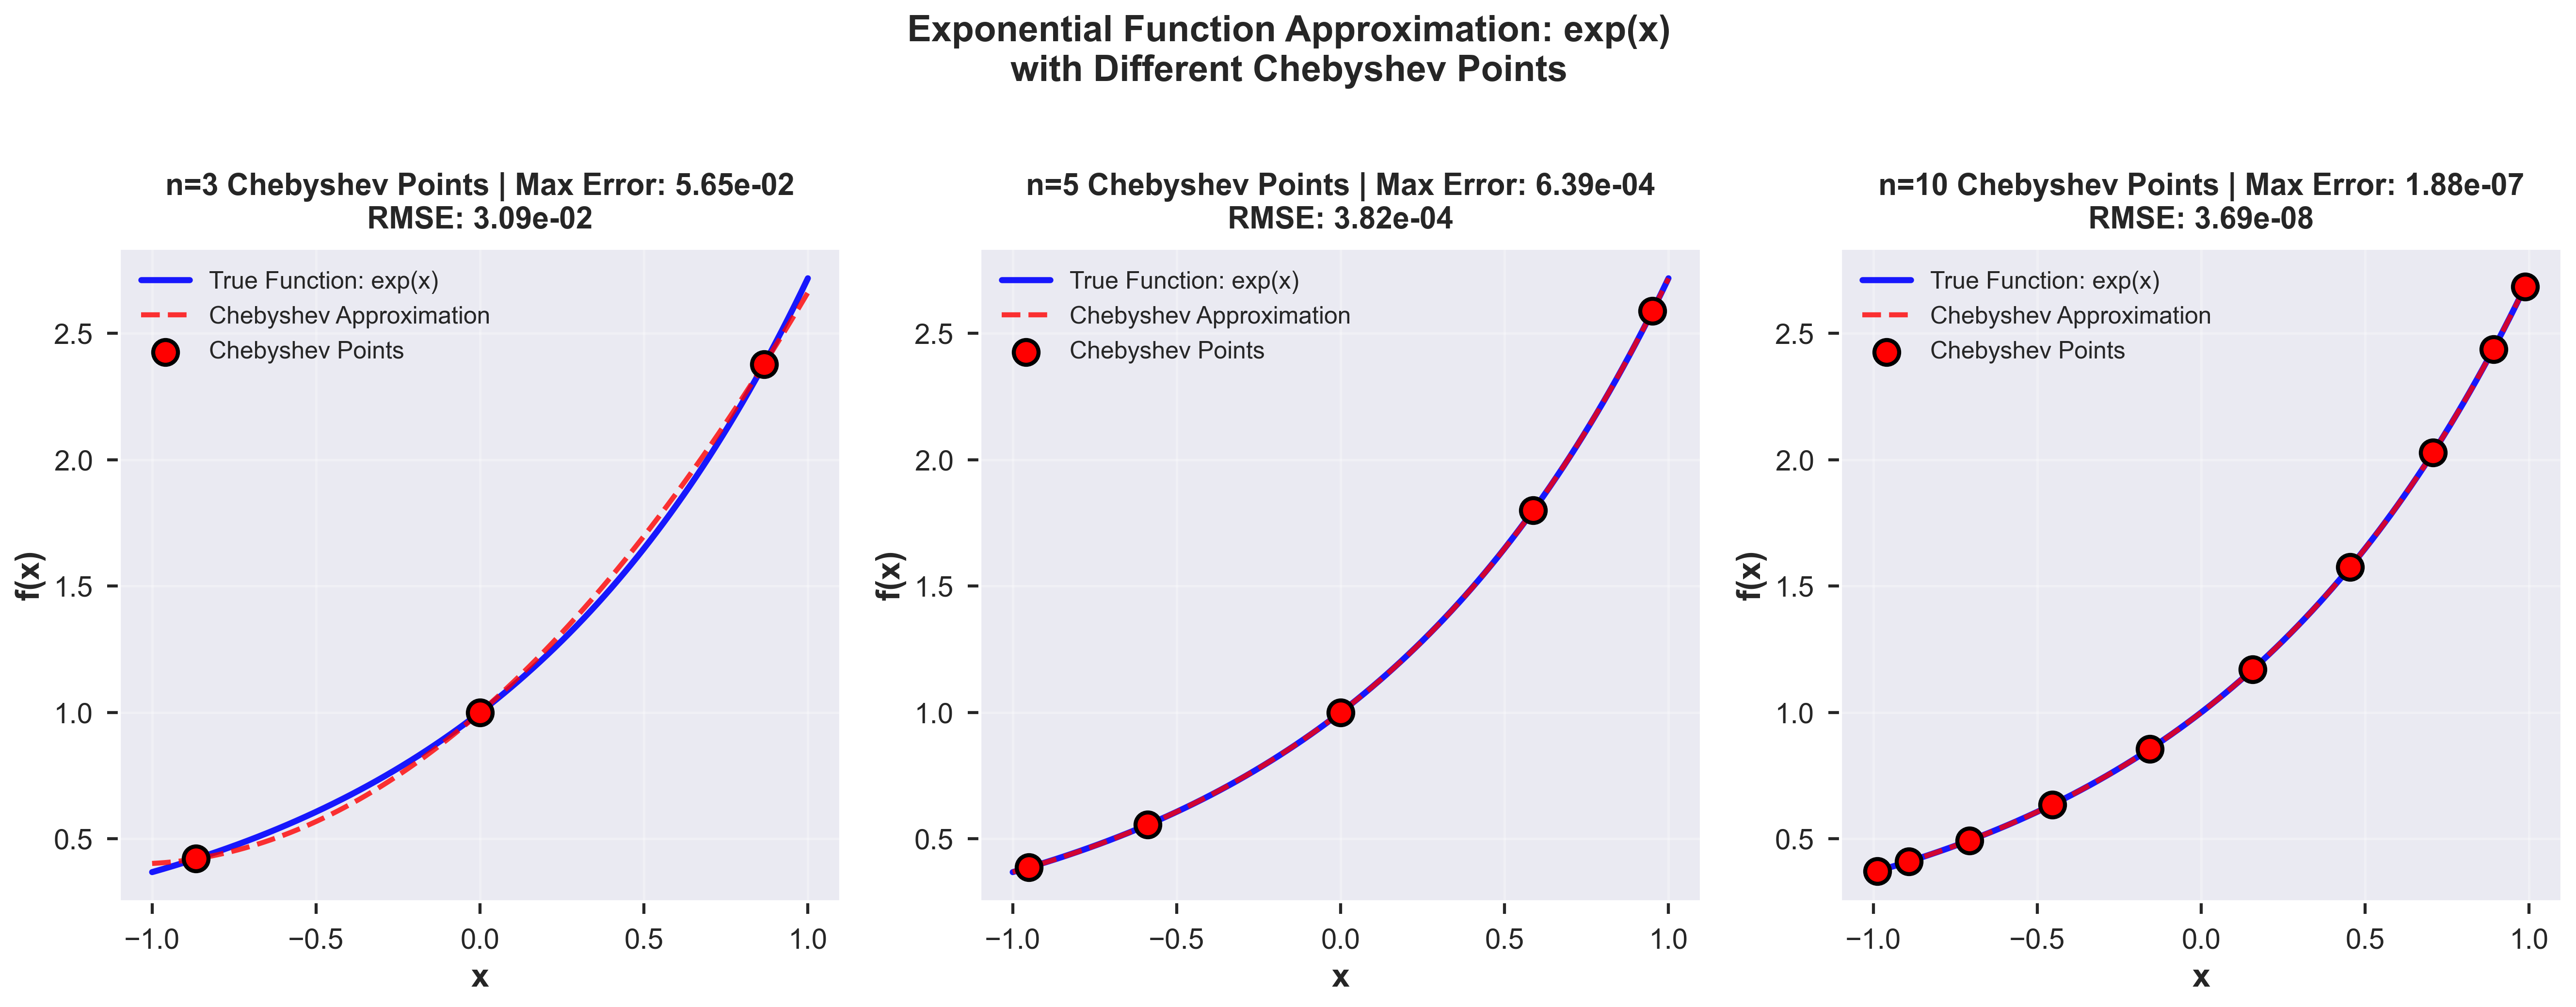
\includegraphics[width=1\textwidth]{figures/teaching/08_exp_approximation.png}
\end{figure}
\end{center}

\vspace{-0.2cm}
\begin{itemize}
    \item With 10 points, maximum error is on the order of $10^{-12}$
\end{itemize}

\end{frame}

\begin{frame}{Chebyshev Approximation: Smooth vs Non-Smooth Functions}

\begin{center}
\begin{figure}
    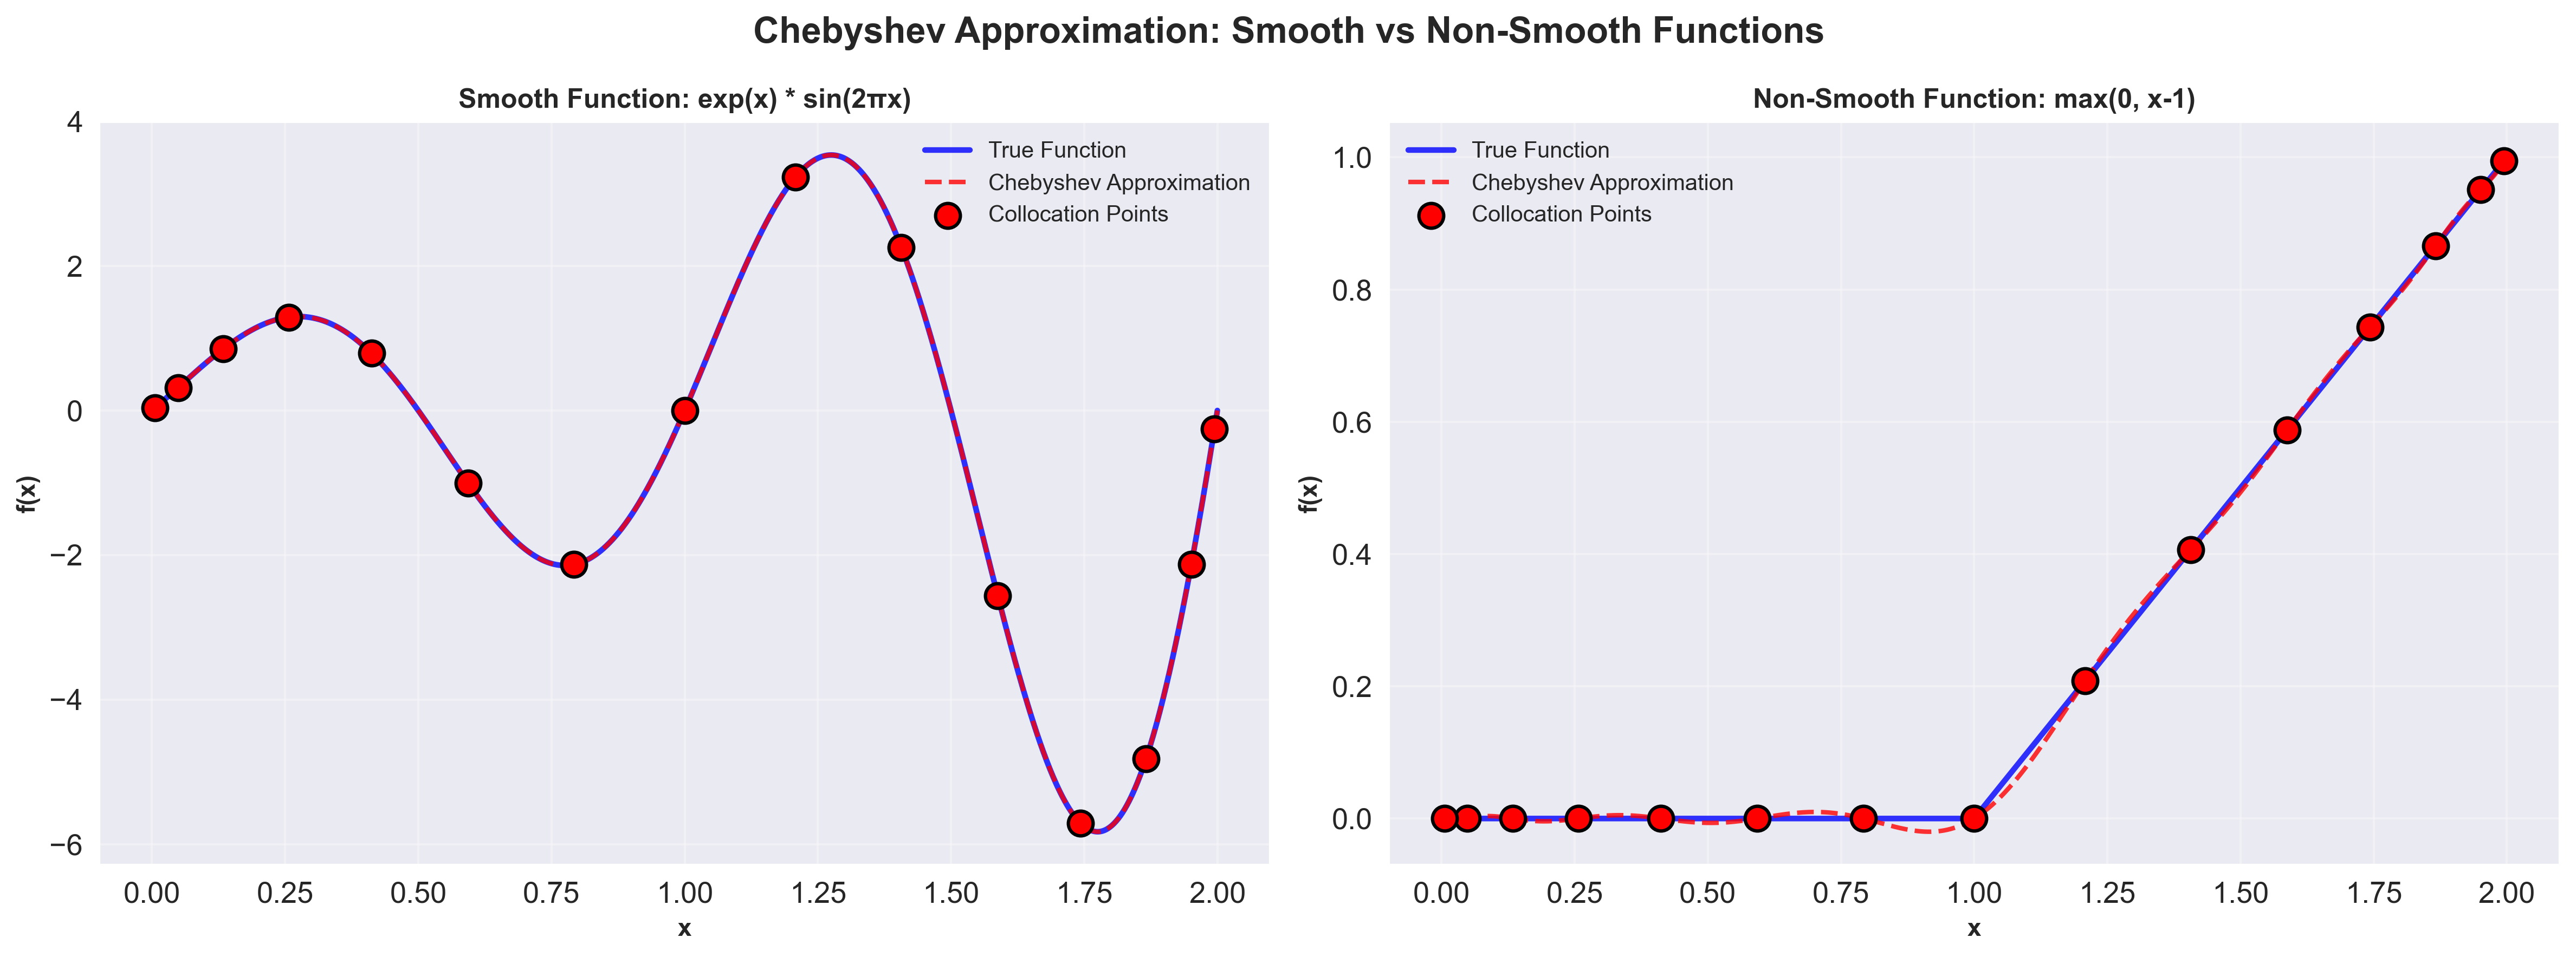
\includegraphics[width=1\textwidth]{figures/teaching/03_smooth_vs_nonsmooth.png}
\end{figure}
\end{center}

\vspace{-0.2cm}
\begin{itemize}
    \item \textbf{Left:} Smooth function $\exp(x) \cdot \sin(2\pi x)$ - Chebyshev approximation is nearly perfect
    \item \textbf{Right:} Non-smooth function $\max(0, x-1)$ - Chebyshev struggles with non-differentiable points
\end{itemize}

\end{frame}


\begin{frame}{Why Chebyshev Over Taylor Polynomials?}

\visible<1->{
    \textbf{\textcolor{darkblue}{Comparison:}}
    \begin{itemize}
        \item \textbf{Taylor polynomials:} Expand around a single point (e.g., center of domain)
        \item \textbf{Chebyshev polynomials:} Distribute approximation error evenly across domain
        \item \textbf{Result:} Chebyshev achieves better \textbf{\textcolor{darkblue}{global accuracy}} with same number of terms
    \end{itemize}
}

\visible<2->{
    \textbf{\textcolor{darkblue}{Key Advantage:}}
    \begin{itemize}
        \item \textbf{\textcolor{darkblue}{Taylor:}} Good near expansion point, deteriorates away from it
        \item \textbf{\textcolor{darkblue}{Chebyshev:}} Optimal nodes minimize maximum error across entire domain
    \end{itemize}
}

\end{frame}

\begin{frame}{Chebyshev vs Taylor Polynomial: Exponential Function}

\begin{center}
\begin{figure}
    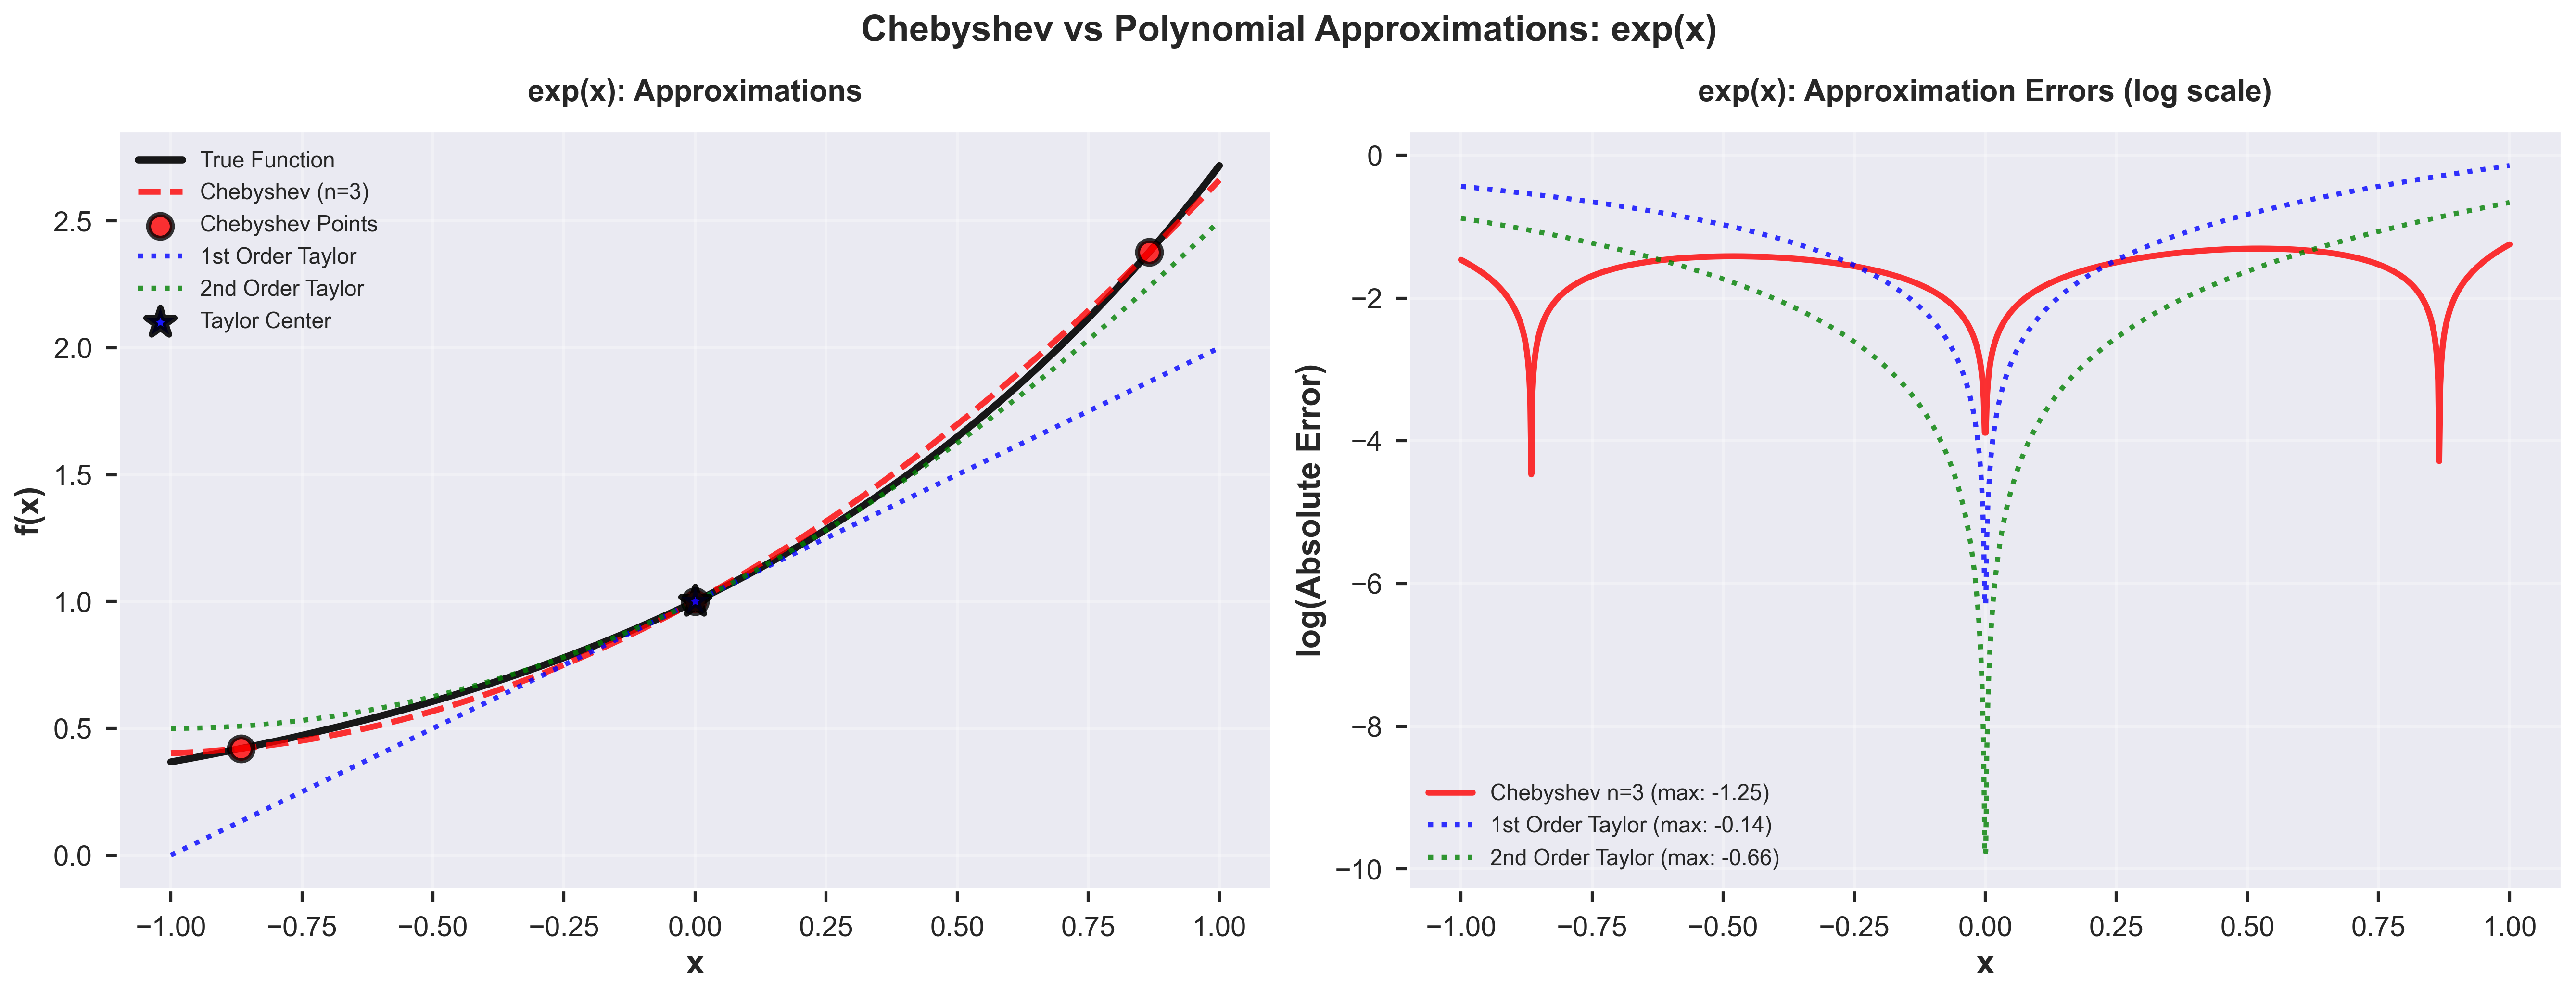
\includegraphics[width=0.98\textwidth]{figures/teaching/09a_chebyshev_vs_polynomial_exp.png}
\end{figure}
\end{center}

\begin{itemize}
    \item \textbf{Left:} Function approximations. \textbf{Right:} Absolute errors (log scale)
    \item \textbf{Log$_{10}$ interpretation:} value $-k$ means absolute error $\sim 10^{-k}$
    \item Chebyshev approximation maintains low error across entire domain
\end{itemize}

\end{frame}

\begin{frame}{Chebyshev Approximation: Curvy Function}

\begin{center}
\begin{figure}
    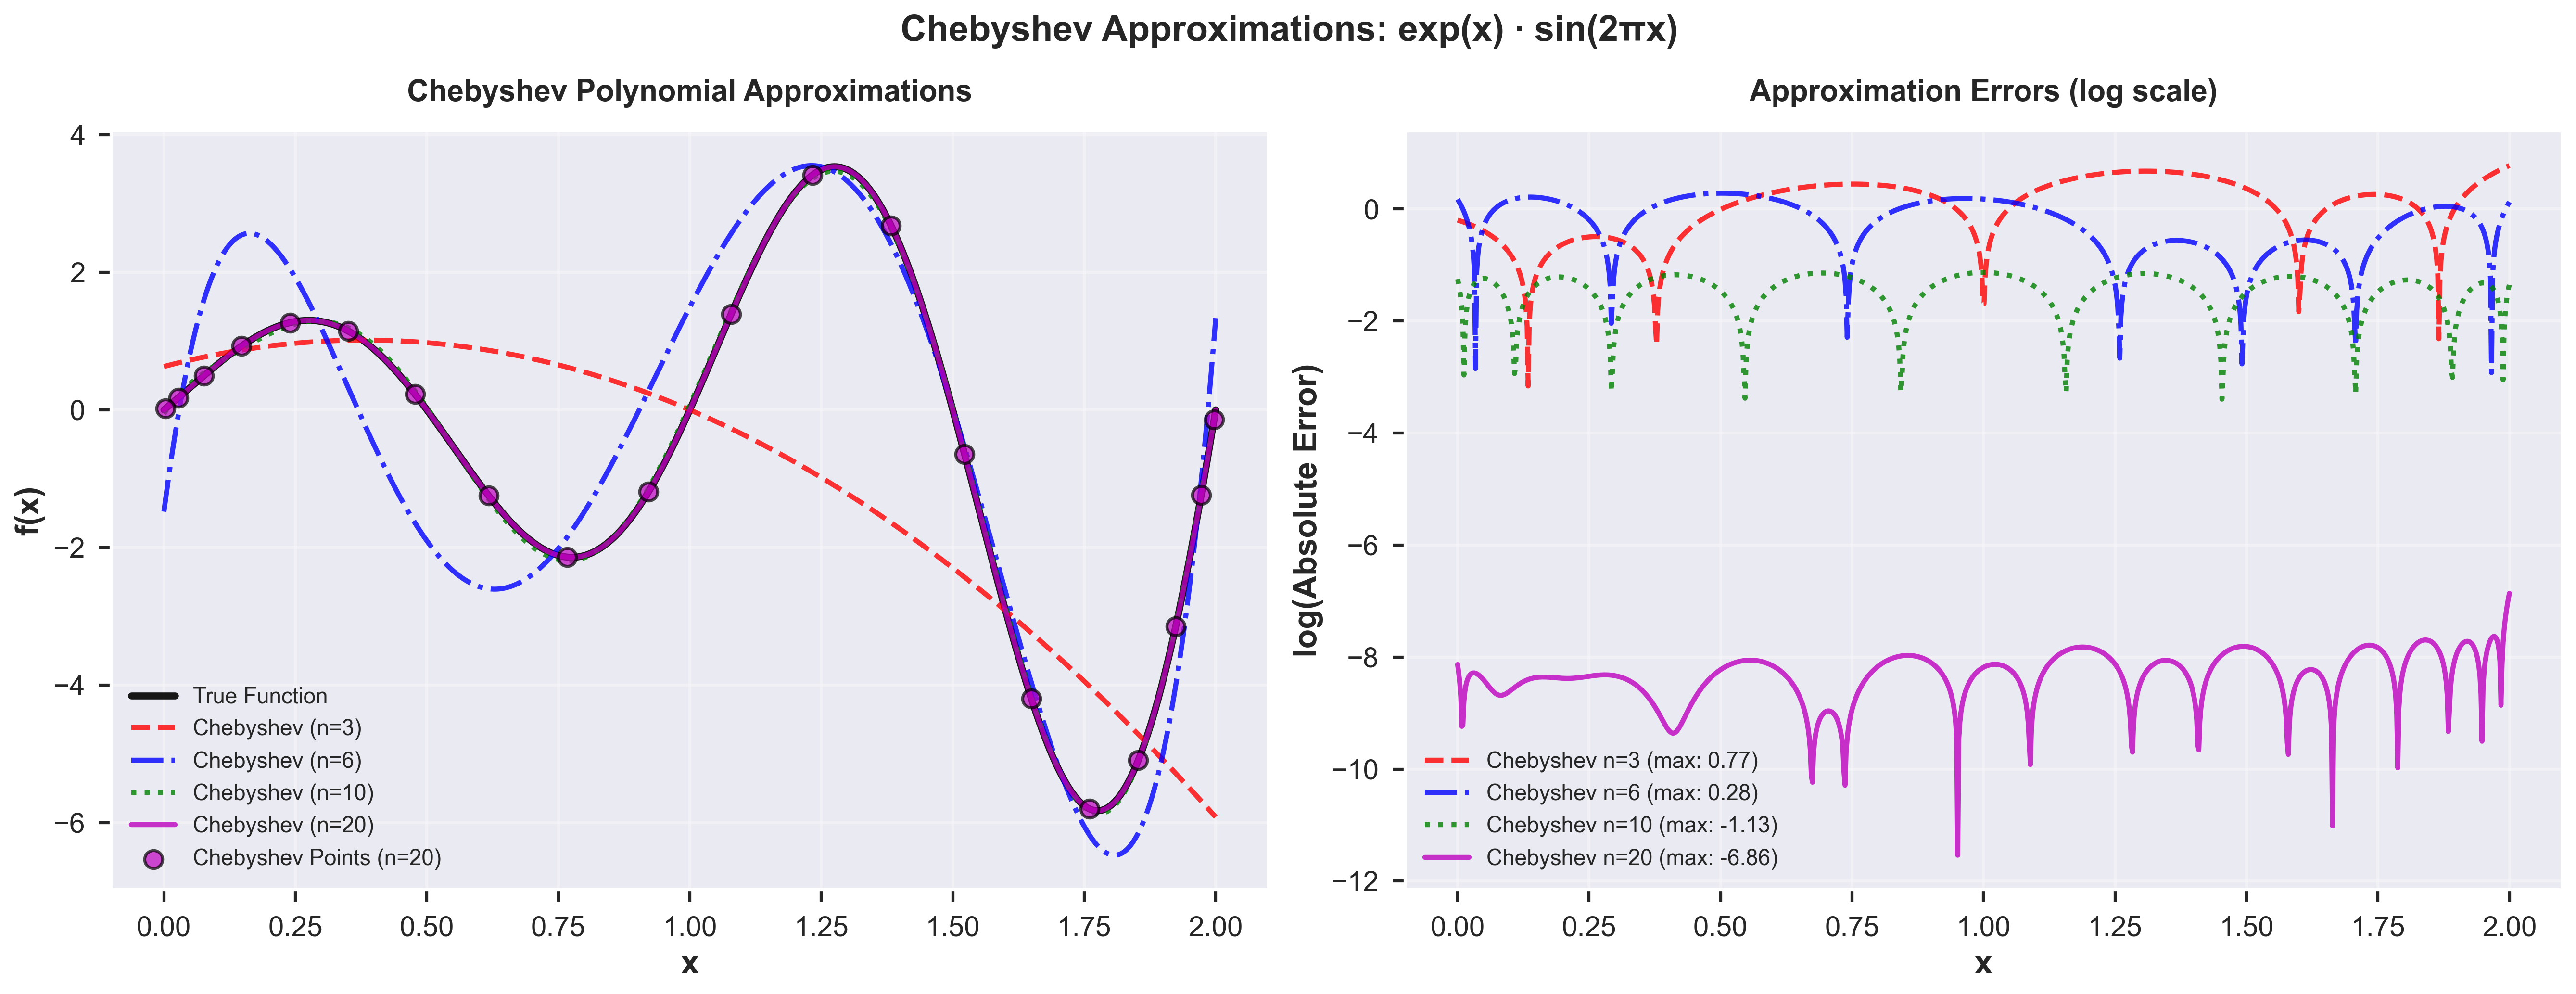
\includegraphics[width=0.98\textwidth]{figures/teaching/14_chebyshev_only.png}
\end{figure}
\end{center}

\begin{itemize}
    \item Very smooth functions require more nodes to approximate well (here 10-20)
    \item Max error: Chebyshev n=3 $\sim 5.92$, n=6 $\sim 1.90$, n=10 $\sim 0.07$
\end{itemize}

\end{frame}

\begin{frame}{Taylor Polynomial Approximation: Curvy Function}

\begin{center}
\begin{figure}
    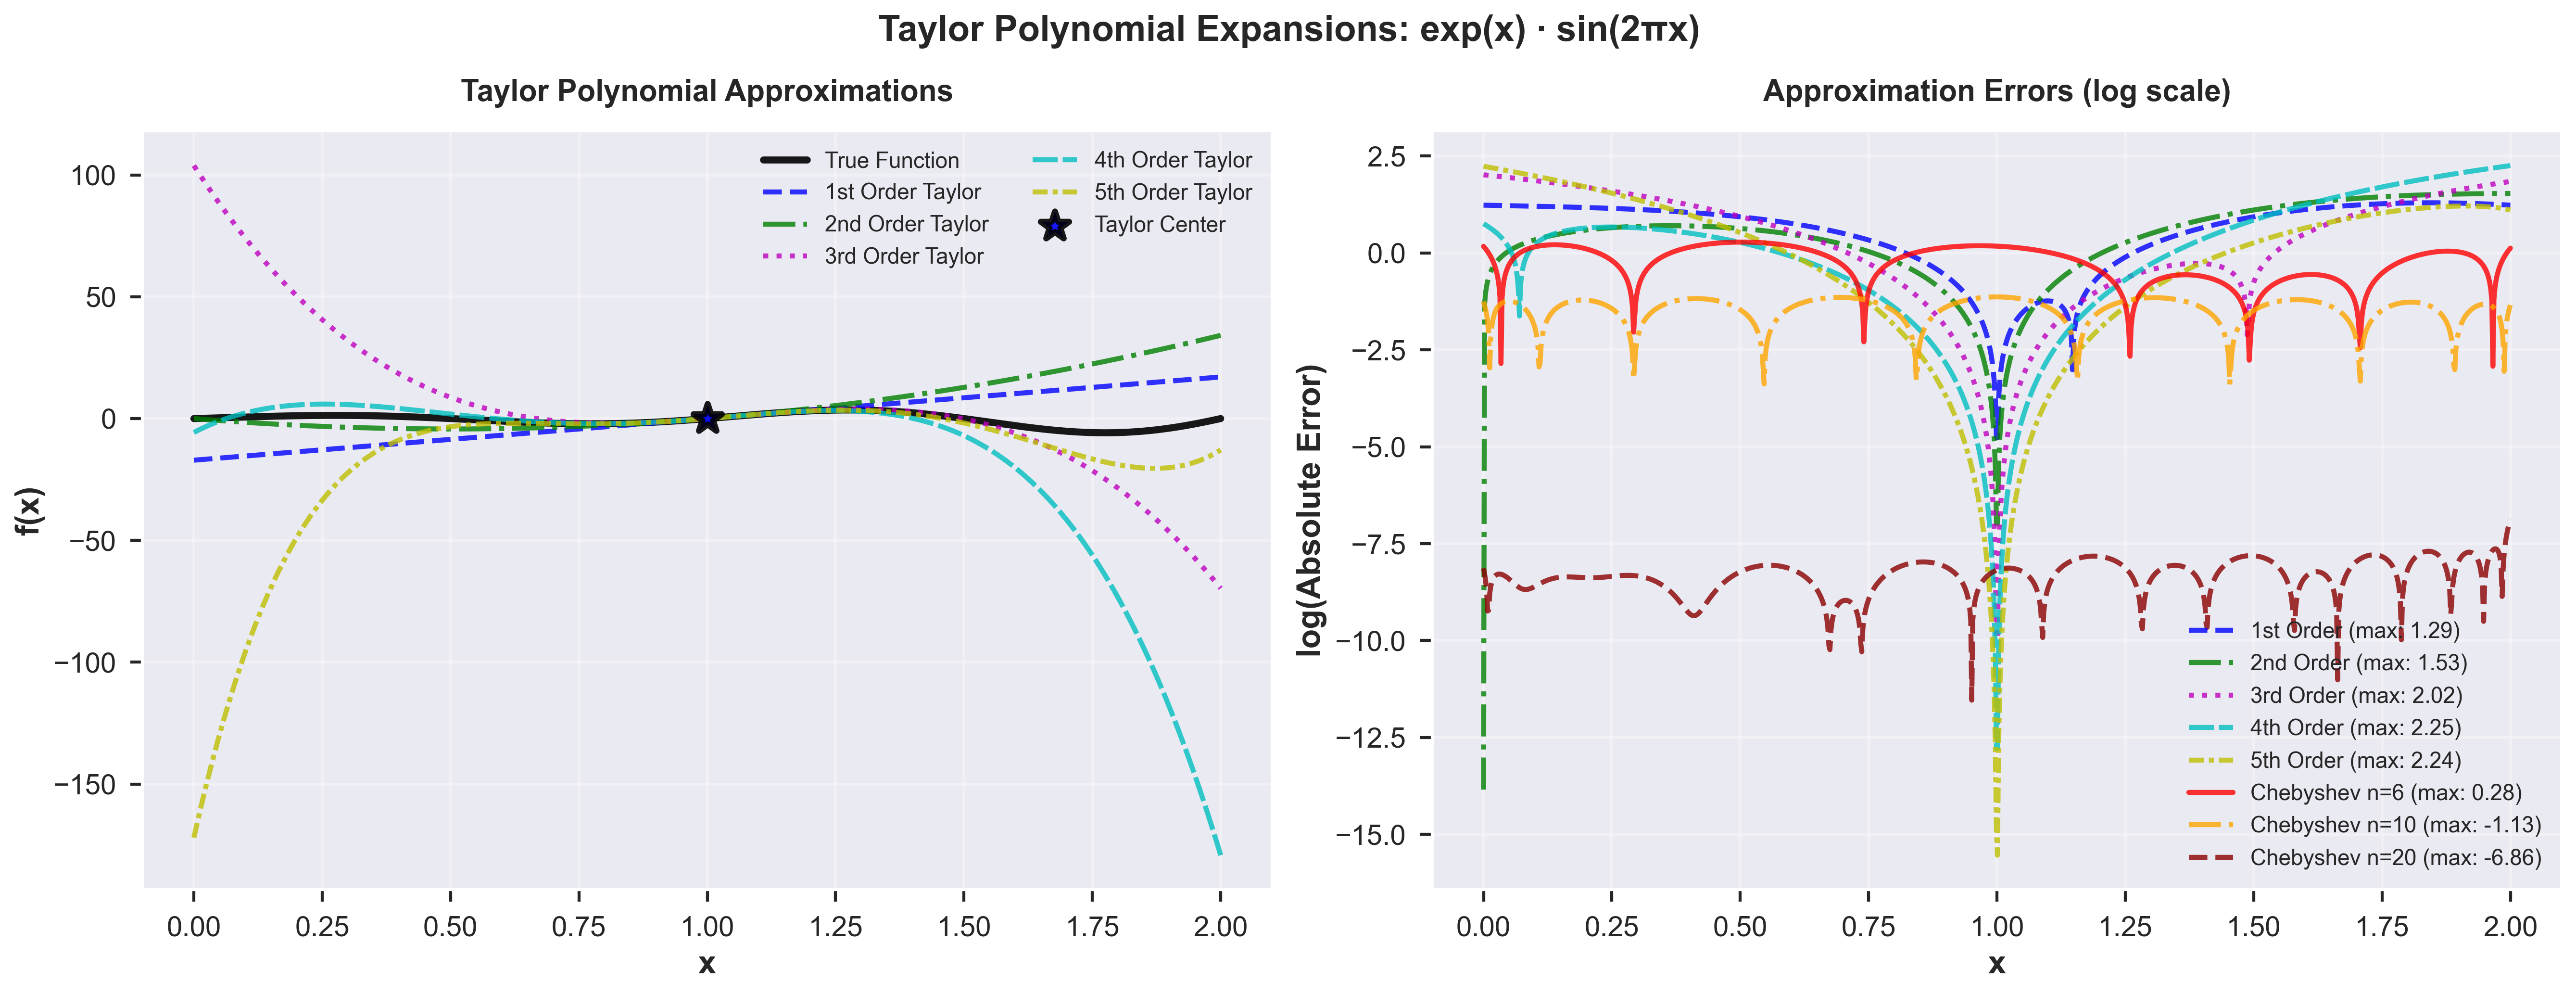
\includegraphics[width=0.98\textwidth]{figures/teaching/13_taylor_expansions_only.png}
\end{figure}
\end{center}

\begin{itemize}
    \item Higher-order terms improve accuracy near expansion point; approximation far from expansion point deteriorates quickly
    \item Max error: Chebyshev n=6 $\sim 1.90$; Taylor 5th $\sim 200.51$
\end{itemize}

\end{frame}


\begin{frame}{Takeaway: Why Chebyshev Wins}

\visible<1->{
    \textbf{\textcolor{darkblue}{Key Insights from Comparison:}}
    \begin{itemize}
        \item \textbf{Error distribution:} Chebyshev minimizes maximum error across entire domain
        \item \textbf{Global approximation:} Unlike Taylor polynomials, error doesn't explode away from a single point
        \item \textbf{Efficiency:} Achieves high accuracy with relatively few points
    \end{itemize}
}

\end{frame}

\setcounter{section}{3}
\section[Example 2: 2D Approximation]{Example 2: Bivariate Approximation}

\begin{frame}{Example 2: Problem Setup}

\visible<1->{
    \textbf{\textcolor{darkblue}{Objective:}} Approximate the function
    \begin{equation*}
    f(x,y) = \exp(x) \cdot \exp(y)
    \end{equation*}
    on the domain $(x,y) \in [0,1] \times [-1,0]$
}

\visible<2->{
    \textbf{\textcolor{darkblue}{Approximation Form (Tensor Product):}}
    \begin{equation*}
    f(x,y) \approx \sum_{n_x=0}^{p_x-1} \sum_{n_y=0}^{p_y-1} \gamma_{n_x n_y} T_{n_x}(\tilde{x}) T_{n_y}(\tilde{y})
    \end{equation*}
    where $\tilde{x}, \tilde{y} \in [-1,1]$ are Chebyshev domains
}

\visible<3->{
    \textbf{\textcolor{darkblue}{Key Choices:}}
    \begin{itemize}
        \item Number of nodes: $n_x$ and $n_y$ (e.g., $n_x = n_y = 10$)
        \item Polynomial orders: $p_x$ and $p_y$ (typically $p_x = n_x$, $p_y = n_y$)
        \item Total coefficients: $p_x \times p_y = 10 \times 10 = 100$
    \end{itemize}
}

\end{frame}

\begin{frame}{Step 1: Choose Grid Parameters and Construct Chebyshev Nodes}

\visible<1->{
    \textbf{\textcolor{darkblue}{Choose:}}
    \begin{itemize}
        \item \textbf{Number of nodes:} $n_x$ and $n_y$ (e.g., $n_x = n_y = 10$)
        \item \textbf{Polynomial orders:} $p_x$ and $p_y$ (typically $p_x = n_x$, $p_y = n_y$)
        \item \textbf{Domains:} 
        \begin{align*}
        x &\in [x_{\min}, x_{\max}] = [0, 1] \\
        y &\in [y_{\min}, y_{\max}] = [-1, 0]
        \end{align*}
    \end{itemize}
}

\visible<2->{
    \vspace{0.2cm}
    \begin{columns}[T]
    \begin{column}{0.48\textwidth}
    \textbf{\textcolor{darkblue}{Chebyshev Nodes in $[-1,1]$:}}
    \begin{equation*}
    \tilde{x}_i = \cos\left(\frac{(2i-1)\pi}{2n_x}\right)
    \end{equation*}
    \begin{equation*}
    \tilde{y}_j = \cos\left(\frac{(2j-1)\pi}{2n_y}\right)
    \end{equation*}
    for $i = 1, \ldots, n_x$, $j = 1, \ldots, n_y$
    \end{column}
    
    \begin{column}{0.48\textwidth}
    \textbf{\textcolor{darkblue}{Transform to Original Domains:}}
    \begin{align*}
    x_i &= \frac{x_{\max} + x_{\min}}{2} + \frac{x_{\max} - x_{\min}}{2} \tilde{x}_i \\
    y_j &= \frac{y_{\max} + y_{\min}}{2} + \frac{y_{\max} - y_{\min}}{2} \tilde{y}_j
    \end{align*}
    \end{column}
    \end{columns}
}



\end{frame}

\begin{frame}{Step 2: Construct Polynomial Matrices and Define Approximation}

\visible<1->{
    \textbf{\textcolor{darkblue}{Approximation Function:}}
    \begin{equation*}
    \hat{f}(x_i, y_j) = \sum_{n_x=0}^{p_x-1} \sum_{n_y=0}^{p_y-1} \gamma_{n_x,n_y} T_{n_x}(\tilde{x}_i) T_{n_y}(\tilde{y}_j)
    \end{equation*}
    where $\boldsymbol{\gamma}$ is a $(p_x \times p_y) \times 1$ column vector: $[\gamma_{0,0}, \gamma_{0,1}, \ldots, \gamma_{0,p_y-1}, \gamma_{1,0}, \ldots, \gamma_{p_x-1,p_y-1}]^T$

    \vspace{0.2cm}
    \begin{columns}[T]
    \begin{column}{0.4\textwidth}
    \textbf{\textcolor{darkblue}{Vectorized Form:}}
    \begin{equation*}
    \begin{bmatrix} \hat{f}(x_1,y_1) \\ \hat{f}(x_1,y_2) \\ \vdots \\ \hat{f}(x_{n_x},y_{n_y}) \end{bmatrix} = \mathbf{T}_x \otimes \mathbf{T}_y\boldsymbol{\gamma}
    \end{equation*}
    \end{column}
    
    \begin{column}{0.6\textwidth}
    \textbf{\textcolor{darkblue}{Polynomial Matrices:}}
    \begin{equation*}
    \mathbf{T}_x = \begin{bmatrix}
    T_0(\tilde{x}_1) & \cdots & T_{p_x-1}(\tilde{x}_1) \\
    \vdots & \ddots & \vdots \\
    T_0(\tilde{x}_{n_x}) & \cdots & T_{p_x-1}(\tilde{x}_{n_x})
    \end{bmatrix}
    \end{equation*}
    \begin{equation*}
    \mathbf{T}_y = \begin{bmatrix}
    T_0(\tilde{y}_1) & \cdots & T_{p_y-1}(\tilde{y}_1) \\
    \vdots & \ddots & \vdots \\
    T_0(\tilde{y}_{n_y}) & \cdots & T_{p_y-1}(\tilde{y}_{n_y})
    \end{bmatrix}
    \end{equation*}
    \end{column}
    \end{columns}
}

\end{frame}

\begin{frame}{Step 2: Construct Polynomial Matrices and Define Approximation}

    \textbf{\textcolor{darkblue}{Linear System:}} $\mathbf{f} = \mathbf{K}_{xy} \boldsymbol{\gamma}$
    
    \vspace{0.2cm}
    \tiny
    \begin{equation*}
    \begin{bmatrix} f(x_1,y_1) \\ f(x_1,y_2) \\ \vdots \\ f(x_1,y_{n_y}) \\ f(x_2,y_1) \\ \vdots \\ f(x_{n_x},y_{n_y}) \end{bmatrix} = \begin{bmatrix}
    T_0(\tilde{x}_1)T_0(\tilde{y}_1) & T_0(\tilde{x}_1)T_1(\tilde{y}_1) & \cdots & T_0(\tilde{x}_1)T_{p_y-1}(\tilde{y}_1) & T_1(\tilde{x}_1)T_0(\tilde{y}_1) & \cdots & T_{p_x-1}(\tilde{x}_1)T_{p_y-1}(\tilde{y}_1) \\
    T_0(\tilde{x}_1)T_0(\tilde{y}_2) & T_0(\tilde{x}_1)T_1(\tilde{y}_2) & \cdots & T_0(\tilde{x}_1)T_{p_y-1}(\tilde{y}_2) & T_1(\tilde{x}_1)T_0(\tilde{y}_2) & \cdots & T_{p_x-1}(\tilde{x}_1)T_{p_y-1}(\tilde{y}_2) \\
    \vdots & \vdots & \ddots & \vdots & \vdots & \ddots & \vdots \\
    T_0(\tilde{x}_1)T_0(\tilde{y}_{n_y}) & T_0(\tilde{x}_1)T_1(\tilde{y}_{n_y}) & \cdots & T_0(\tilde{x}_1)T_{p_y-1}(\tilde{y}_{n_y}) & T_1(\tilde{x}_1)T_0(\tilde{y}_{n_y}) & \cdots & T_{p_x-1}(\tilde{x}_1)T_{p_y-1}(\tilde{y}_{n_y}) \\
    T_0(\tilde{x}_2)T_0(\tilde{y}_1) & T_0(\tilde{x}_2)T_1(\tilde{y}_1) & \cdots & T_0(\tilde{x}_2)T_{p_y-1}(\tilde{y}_1) & T_1(\tilde{x}_2)T_0(\tilde{y}_1) & \cdots & T_{p_x-1}(\tilde{x}_2)T_{p_y-1}(\tilde{y}_1) \\
    \vdots & \vdots & \ddots & \vdots & \vdots & \ddots & \vdots \\
    T_0(\tilde{x}_{n_x})T_0(\tilde{y}_1) & T_0(\tilde{x}_{n_x})T_1(\tilde{y}_1) & \cdots & T_0(\tilde{x}_{n_x})T_{p_y-1}(\tilde{y}_1) & T_1(\tilde{x}_{n_x})T_0(\tilde{y}_1) & \cdots & T_{p_x-1}(\tilde{x}_{n_x})T_{p_y-1}(\tilde{y}_1) \\
    \vdots & \vdots & \ddots & \vdots & \vdots & \ddots & \vdots \\
    T_0(\tilde{x}_{n_x})T_0(\tilde{y}_{n_y}) & T_0(\tilde{x}_{n_x})T_1(\tilde{y}_{n_y}) & \cdots & T_0(\tilde{x}_{n_x})T_{p_y-1}(\tilde{y}_{n_y}) & T_1(\tilde{x}_{n_x})T_0(\tilde{y}_{n_y}) & \cdots & T_{p_x-1}(\tilde{x}_{n_x})T_{p_y-1}(\tilde{y}_{n_y})
    \end{bmatrix} \begin{bmatrix} \gamma_{0,0} \\ \gamma_{0,1} \\ \vdots \\ \gamma_{0,p_y-1} \\ \gamma_{1,0} \\ \vdots \\ \gamma_{p_x-1,p_y-1} \end{bmatrix}
    \end{equation*}
    \normalsize

\end{frame}

\begin{frame}{Step 3: Solve for Optimal Coefficients (2D)}

\visible<1->{
    \textbf{\textcolor{darkblue}{Linear System:}}
    \begin{equation*}
    \mathbf{f} = \mathbf{K}_{xy} \boldsymbol{\gamma}
    \end{equation*}
    where:
    \begin{itemize}
        \item $\mathbf{f}$ is $(n_x \times n_y) \times 1$ column vector: $[f(x_1,y_1), f(x_1,y_2), \ldots, f(x_1,y_{n_y}), f(x_2,y_1), \ldots, f(x_{n_x},y_{n_y})]^T$
        \item $\boldsymbol{\gamma}$ is $(p_x \times p_y) \times 1$ column vector: $[\gamma_{0,0}, \gamma_{0,1}, \ldots, \gamma_{0,p_y-1}, \gamma_{1,0}, \ldots, \gamma_{p_x-1,p_y-1}]^T$
        \item Each row of $\mathbf{K}_{xy}$ multiplies $\boldsymbol{\gamma}$ to give function value at that grid point
    \end{itemize}

    \vspace{0.2cm}
    \textbf{\textcolor{darkblue}{Solution:}}
    \begin{equation*}
    \boldsymbol{\gamma}^* = (\mathbf{K}_{xy}^T \mathbf{K}_{xy})^{-1} \mathbf{K}_{xy}^T \mathbf{f}
    \end{equation*}
    For exactly identified system ($n_x = p_x$, $n_y = p_y$): $\boldsymbol{\gamma}^* = \mathbf{K}_{xy}^{-1} \mathbf{f}$
}

\end{frame}

\begin{frame}{Step 4: Evaluate Approximation at New Points (2D)}

\visible<1->{
    \textbf{\textcolor{darkblue}{Key Advantage:}} Once we have $\boldsymbol{\gamma}^*$, we have an \textbf{approximator}—no interpolation needed!
    
    \textbf{\textcolor{darkblue}{To evaluate at arbitrary points $(x_{\text{new}}, y_{\text{new}})$:}}
    \begin{itemize}
        \item Transform to Chebyshev domains: $\tilde{x}_{\text{new}}$, $\tilde{y}_{\text{new}}$
        \item Compute tensor product matrix $\mathbf{K}_{\text{new}}$ at new points
        \item Evaluate: $\hat{f}(x_{\text{new}}, y_{\text{new}}) = \boldsymbol{\gamma}^{*\prime} \mathbf{K}_{\text{new}}$
    \end{itemize}
}

\visible<2->{
    \textbf{\textcolor{darkblue}{Simple Example:}} Suppose we want $f(0.3, 0.7)$ but only know function values at Chebyshev nodes.
    \begin{itemize}
        \item \textbf{Without approximator:} Need interpolation (e.g., bilinear, spline)
        \item \textbf{With Chebyshev approximator:} Just evaluate $\hat{f}(0.3, 0.7) = \boldsymbol{\gamma}^{*\prime} \mathbf{K}_{(0.3,0.7)}$ directly
    \end{itemize}
}

\end{frame}

\begin{frame}{Example 2: Results with 3×3 Chebyshev Points}

\begin{center}
\begin{figure}
    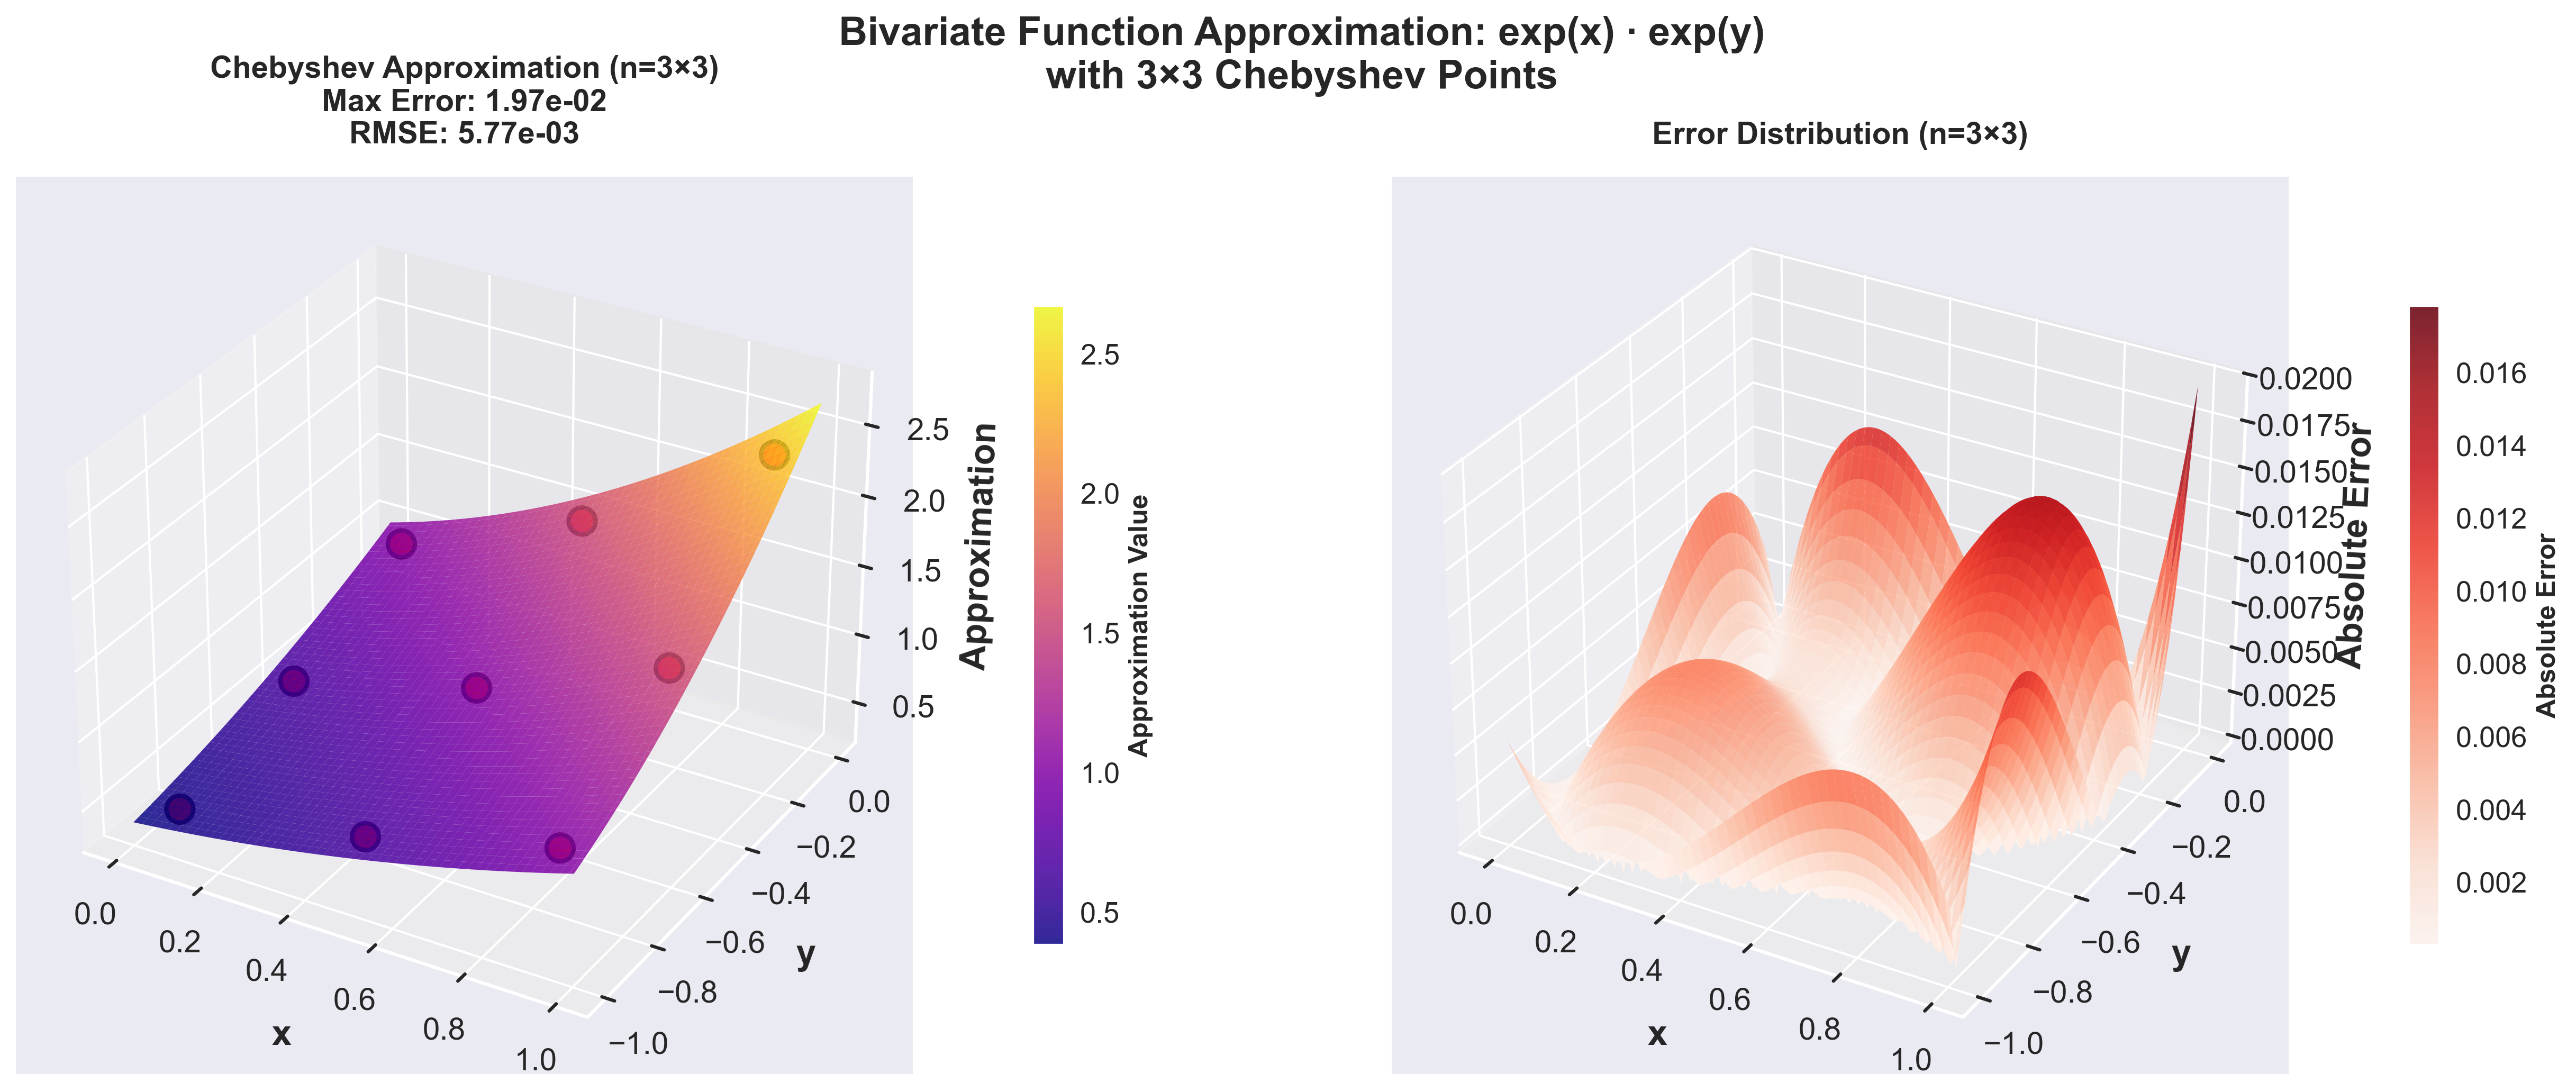
\includegraphics[width=0.8\textwidth]{figures/teaching/05_bivariate_approximation_3points.png}
\end{figure}
\end{center}

\begin{itemize}
    \item \textbf{Left:} Chebyshev approximation with $3 \times 3 = 9$ collocation points (red dots)
    \item \textbf{Right:} Absolute error distribution (maximum error: $1.97 \times 10^{-2}$)
\end{itemize}

\end{frame}

\begin{frame}{Example 2: Results with 5×5 Chebyshev Points}

\begin{center}
\begin{figure}
    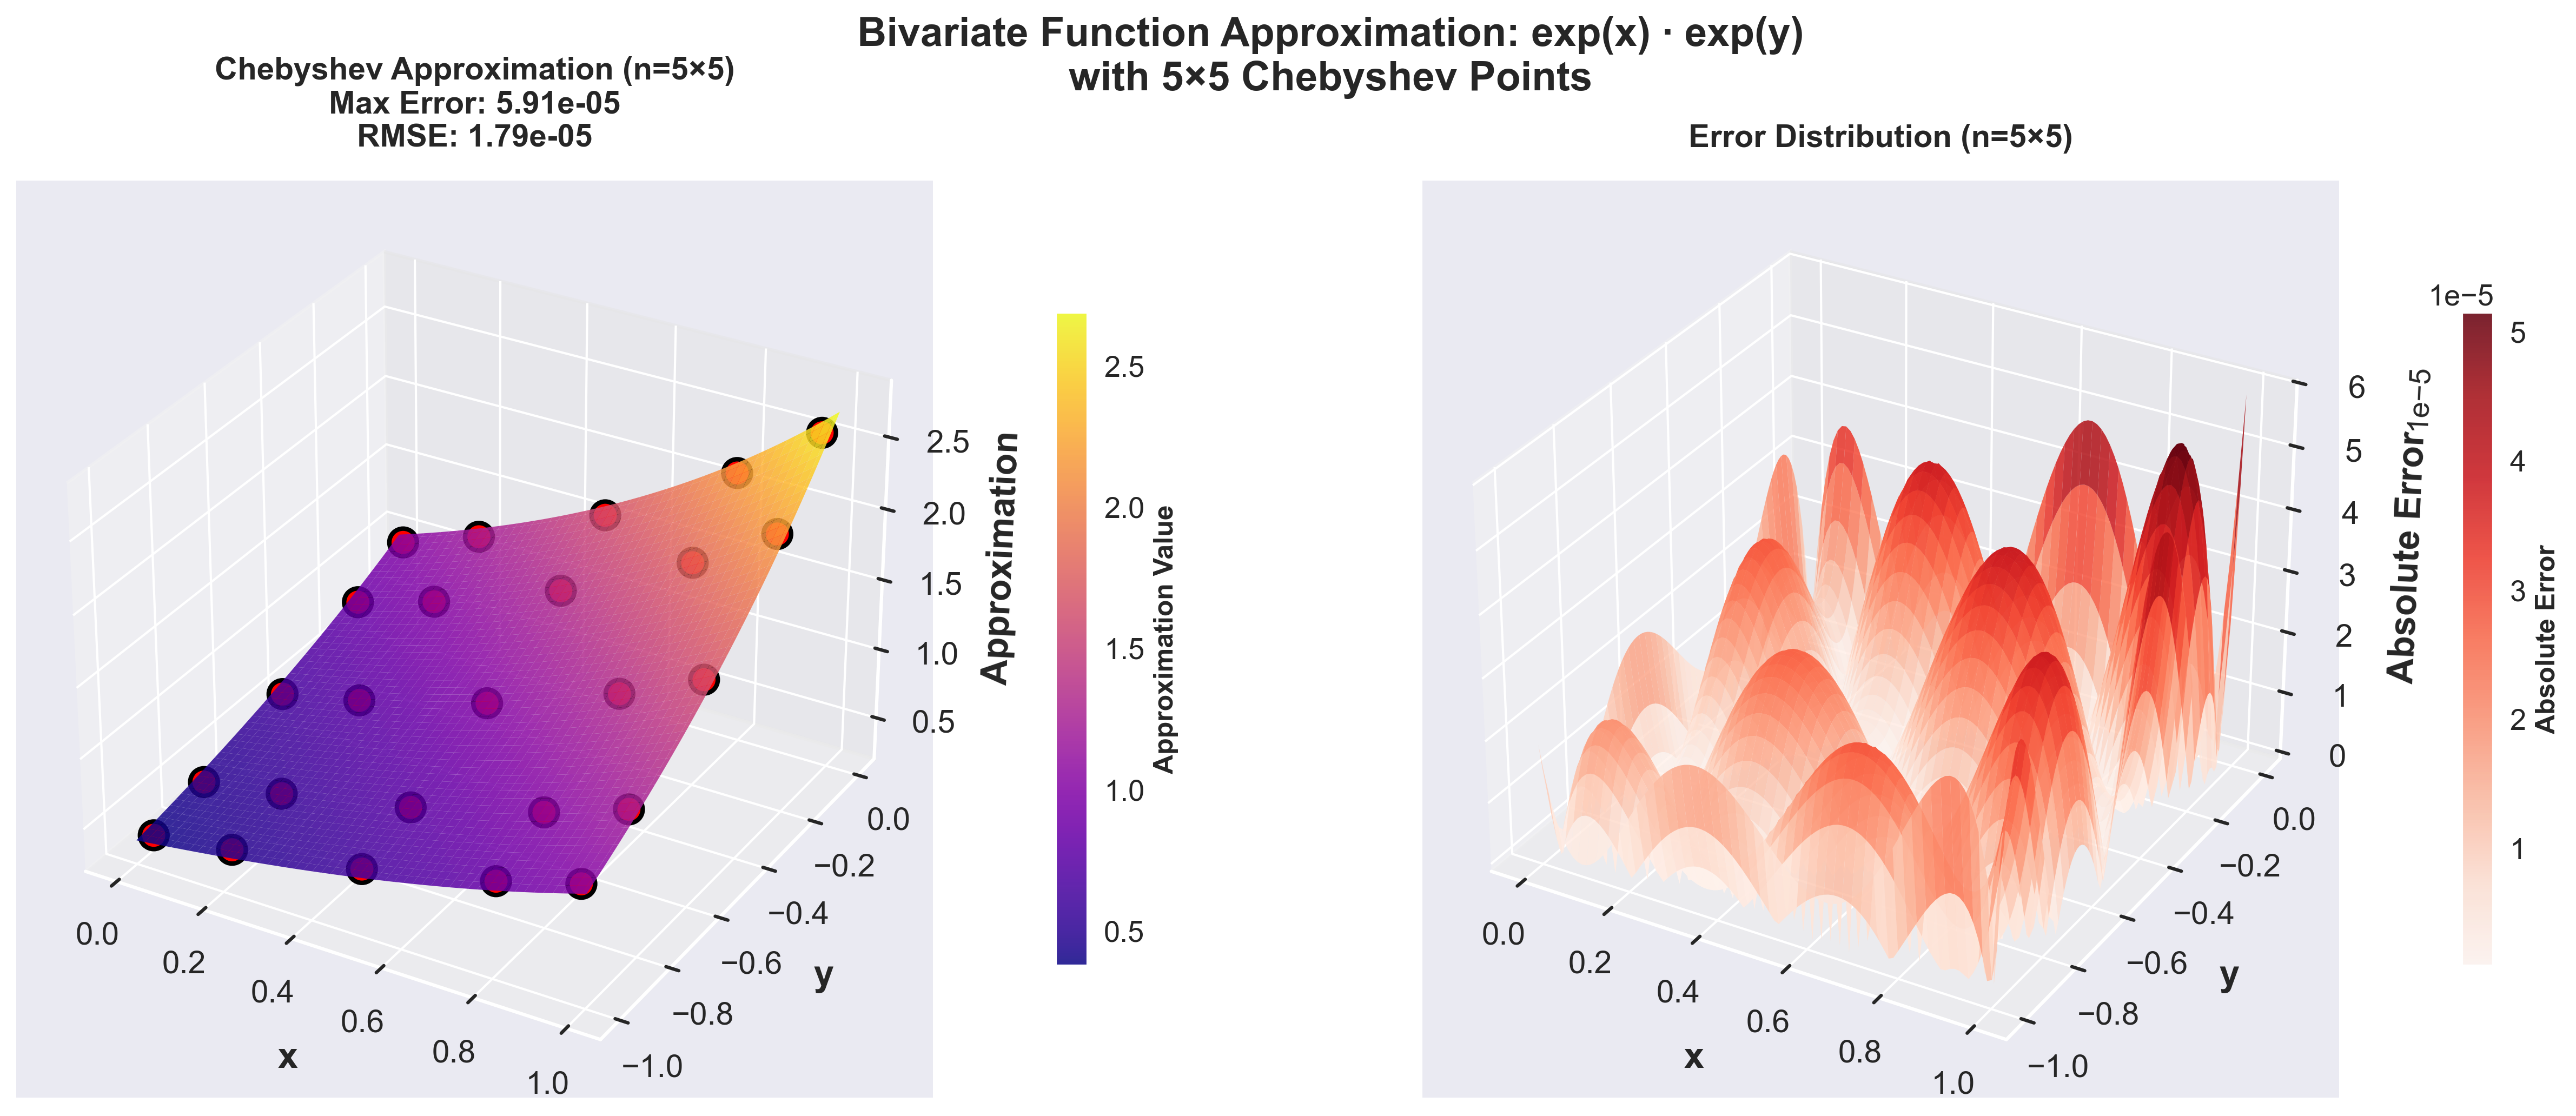
\includegraphics[width=0.8\textwidth]{figures/teaching/05_bivariate_approximation_5points.png}
\end{figure}
\end{center}

\begin{itemize}
    \item \textbf{Left:} Chebyshev approximation with $5 \times 5 = 25$ collocation points (red dots)
    \item \textbf{Right:} Absolute error distribution (maximum error: $5.91 \times 10^{-5}$)
\end{itemize}

\end{frame}

\begin{frame}{Example 2: Results with 10×10 Chebyshev Points}

\begin{center}
\begin{figure}
    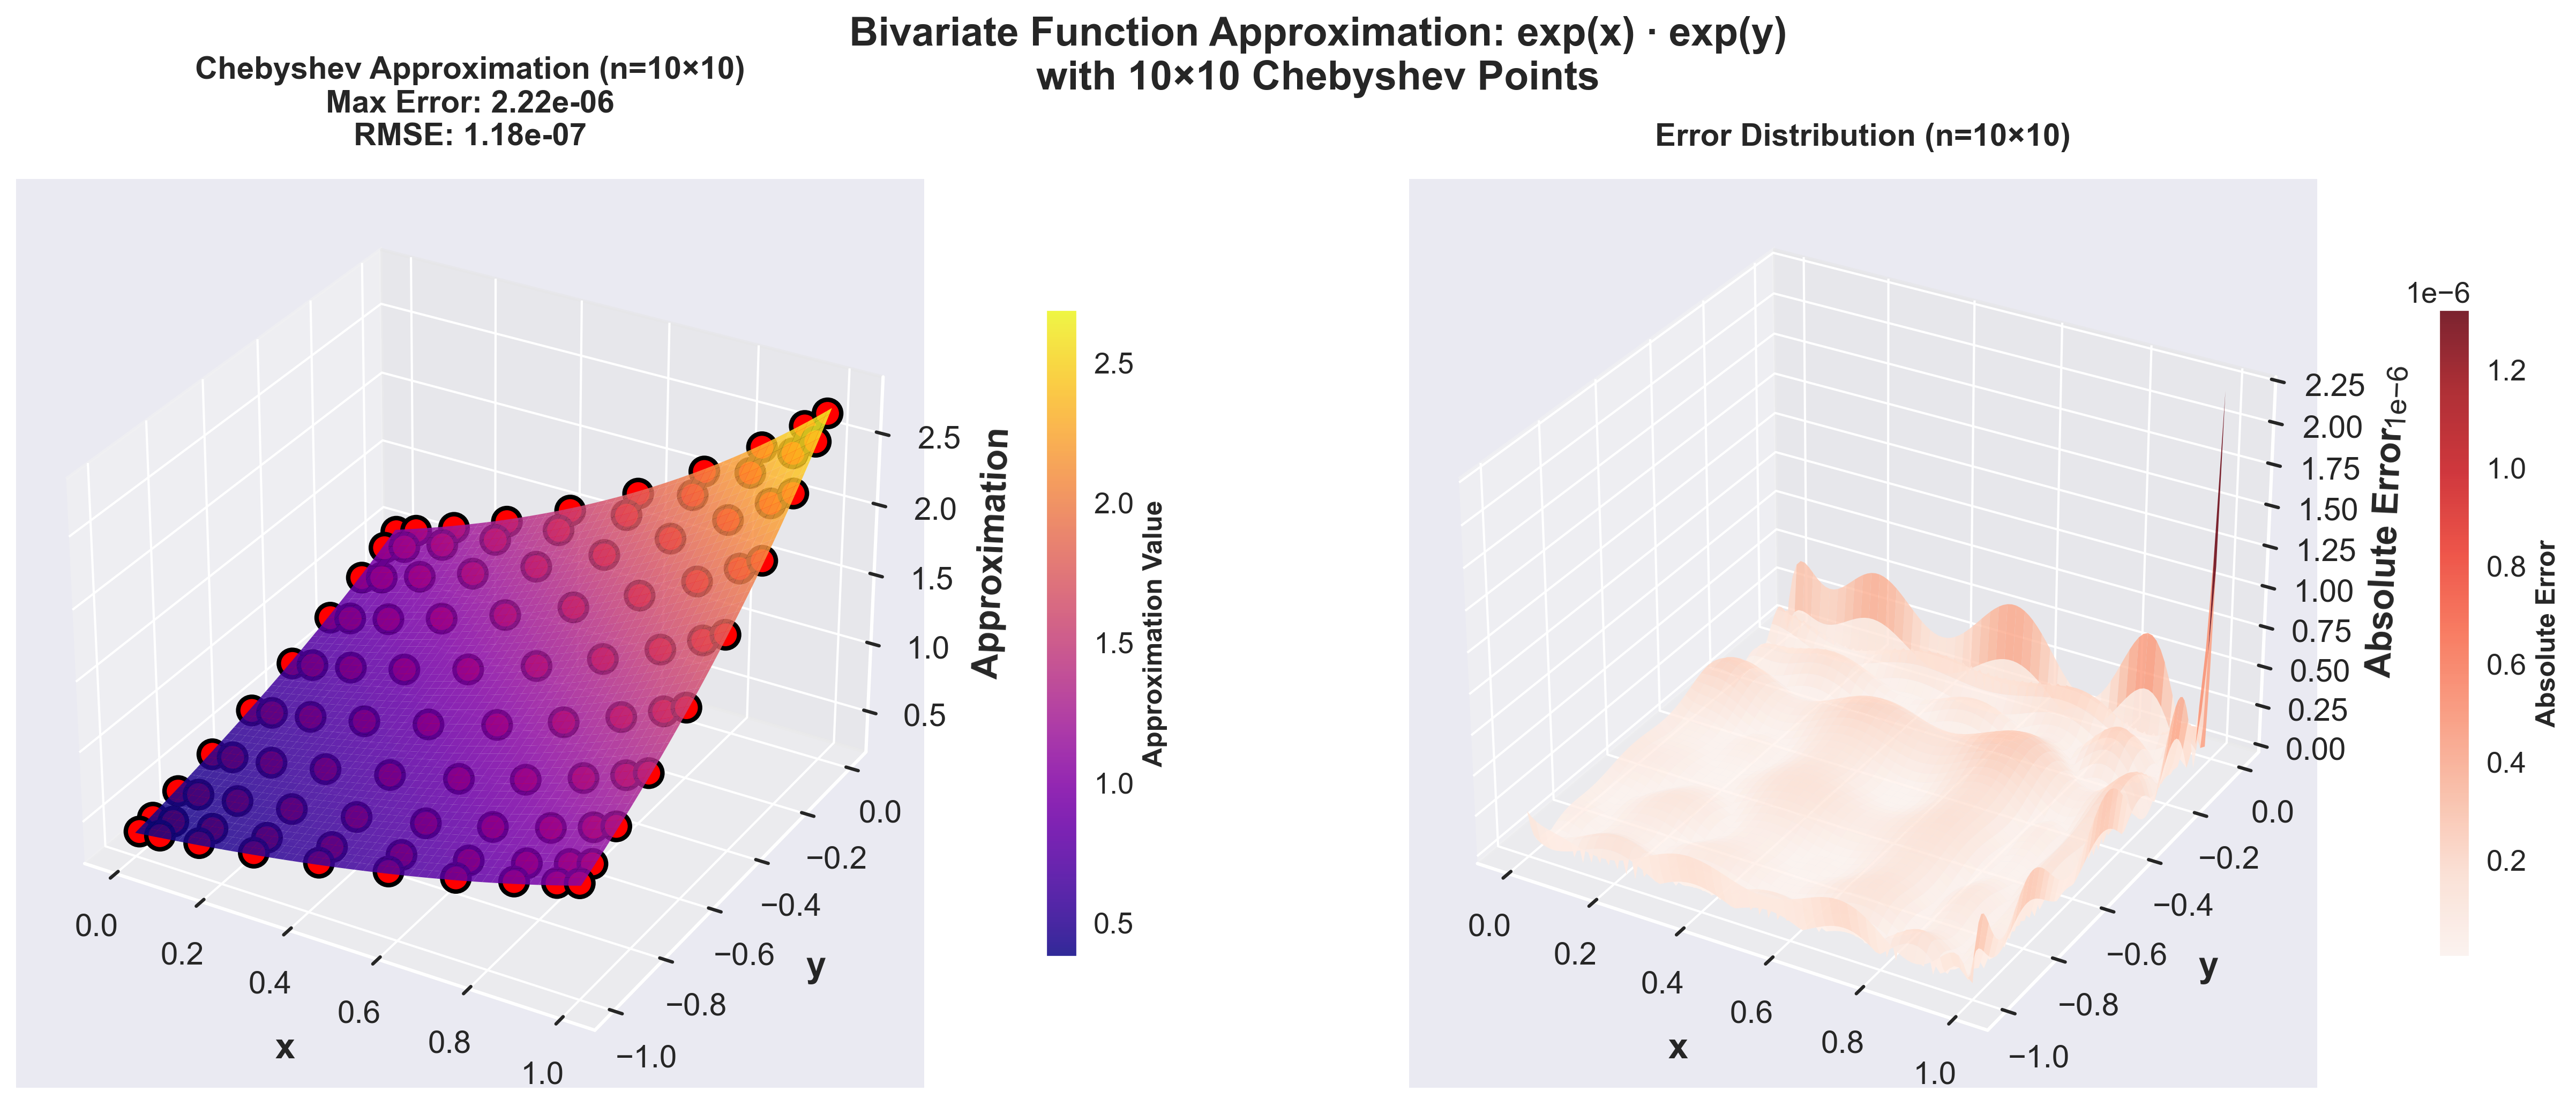
\includegraphics[width=0.8\textwidth]{figures/teaching/05_bivariate_approximation_10points.png}
\end{figure}
\end{center}

\begin{itemize}
    \item \textbf{Left:} Chebyshev approximation with $10 \times 10 = 100$ collocation points (red dots)
    \item \textbf{Right:} Absolute error distribution (maximum error: $2.22 \times 10^{-6}$)
\end{itemize}

\end{frame}



\setcounter{section}{4}
\section[Solving NGM]{Solving the Neoclassical Growth Model}

\begin{frame}{Back to the Neoclassical Growth Model}

\visible<1->{
    \textbf{\textcolor{darkblue}{Now we apply what we learned:}}
    \begin{itemize}
        \item We know how to approximate functions using Chebyshev polynomials (Examples 1 \& 2)
        \item We know how to choose grids, construct polynomial matrices, and solve for coefficients
        \item \textbf{Now:} Apply these techniques to solve the Neoclassical Growth Model
    \end{itemize}
    
    \textbf{\textcolor{darkblue}{Key Difference:}}
    \begin{itemize}
        \item \textbf{Examples:} We knew the true function $f(x)$ and minimized approximation error
        \item \textbf{NGM:} We don't know the true function, but we know \textbf{equilibrium conditions}
        \item \textbf{Solution:} Find coefficients that make equilibrium conditions hold (approximately)
    \end{itemize}
    
    \textbf{\textcolor{darkblue}{Objective:}} Find consumption function $c(z,K)$ such that Euler equation holds:
    \begin{equation*}
    1 = \mathbb{E}_S\left[\beta \frac{c(z,K)}{c(z',K')} \left(\alpha \frac{y(z',K')}{K'} + 1 - \delta\right)\right]
    \end{equation*}
}

\end{frame}

\begin{frame}{Step 1: Approximate Consumption Policy (Part 1)}

\visible<1->{
    \textbf{\textcolor{darkblue}{Setup:}}
    \begin{itemize}
        \item Nodes: $n_z$ (productivity), $n_k$ (capital); orders: $p_z = n_z$, $p_k = n_k$
        \item Domains: $z \in [z_l, z_u]$, $K \in [0.5K_{ss}, 1.5K_{ss}]$
    \end{itemize}
    
    \textbf{\textcolor{darkblue}{Chebyshev Nodes (in $[-1,1]$):}}
    \begin{align*}
    \tilde{z}_j &= \cos\left(\frac{(2j-1)\pi}{2n_z}\right), \quad j = 1, \ldots, n_z \\
    \tilde{K}_j &= \cos\left(\frac{(2j-1)\pi}{2n_k}\right), \quad j = 1, \ldots, n_k
    \end{align*}
    
    \textbf{\textcolor{darkblue}{Transform to Original Domains:}}
    \begin{align*}
    z_j &= \frac{z_l + z_u}{2} + \frac{z_u - z_l}{2} \cdot \tilde{z}_j, \quad K_j = \frac{K_l + K_u}{2} + \frac{K_u - K_l}{2} \cdot \tilde{K}_j
    \end{align*}
}

\end{frame}

\begin{frame}{Step 1: Approximate Consumption Policy (Part 2)}

\visible<1->{
    \textbf{\textcolor{darkblue}{Approximation Form:}}
    \begin{equation*}
    c(z,K) = \sum_{i=0}^{n_z-1} \sum_{j=0}^{n_k-1} \gamma_{ij} T_i(\tilde{z}) T_j(\tilde{K})
    \end{equation*}
    where $\tilde{z} = 2\frac{z - z_l}{z_u - z_l} - 1$, $\tilde{K} = 2\frac{K - K_l}{K_u - K_l} - 1$ map to $[-1,1]$
    
}

\end{frame}

\begin{frame}{Step 2: Compute Other Functions}
    \small
    
    \textbf{\textcolor{darkblue}{Given $c(z,K;\gamma)$, compute other objects from equilibrium conditions:}}
    
    \begin{enumerate}
      \item \textbf{\textcolor{darkblue}{Labor (intratemporal FOC):}}
      \[
      \ell(z,K) \;=\; \left[\frac{(1-\alpha)\,e^{z} K^{\alpha}}{\chi\, c(z,K;\gamma)}\right]^{\frac{\nu}{1+\alpha\nu}}
      \]
    
      \item \textbf{\textcolor{darkblue}{Output:}}
      \[
      y(z,K) \;=\; e^{z}\, K^{\alpha}\, \ell(z,K)^{\,1-\alpha}
      \]
    
      \item \textbf{\textcolor{darkblue}{Next-Period Capital (resource constraint):}}
      \[
      K'(z,K) \;=\; y(z,K) \;-\; c(z,K;\gamma) \;+\; (1-\delta)\,K
      \]
    \end{enumerate}
    
    \vspace{0.6em}
    \textbf{\textcolor{darkblue}{Constraints:}}
    \begin{itemize}
      \item \textbf{Mapped capital (clip in Chebyshev domain):}
      \[
      \tilde K'(z,K) \;=\; \max\!\left\{-1,\; \min\!\left\{1,\;
      \frac{2K'(z,K) - (K_\ell + K_u)}{K_u - K_\ell}
      \right\}\right\}
      \]
      \item \textbf{Consumption positivity:} \quad \(c(z,K;\gamma) > 0\)
    \end{itemize}
    
    \end{frame}
    

\begin{frame}{Step 3: Compute Euler Residual}

\visible<1->{
    \textbf{\textcolor{darkblue}{Euler Equation:}}
    \begin{equation*}
    1 = \mathbb{E}_S\left[\beta \frac{c(z,K;\gamma)}{c(z',K';\gamma)} \left(\alpha \frac{y(z',K')}{K'} + 1 - \delta\right)\right]
    \end{equation*}
    
    \textbf{\textcolor{darkblue}{Productivity Process:}} $z' = \rho_z z + \xi \varepsilon$ where $\varepsilon \sim N(0, \sigma_z^2)$
    
    \textbf{\textcolor{darkblue}{Gauss-Hermite Quadrature:}} (Numerical integration)
    \begin{equation*}
    \mathbb{E}_S[\cdot] = \frac{1}{\sqrt{\pi}} \sum_{i=1}^{n_q} w_i \left[\beta \frac{c(z,K;\gamma)}{c(\sqrt{2}\sigma_z \omega_i + \rho_z z, K';\gamma)} \left(\alpha e^{\sqrt{2}\sigma_z \omega_i + \rho_z z} K'^{\alpha-1} \ell(\cdot)^{1-\alpha} + 1 - \delta\right)\right]
    \end{equation*}
    where $\omega_i, w_i$ are quadrature nodes and weights
    
    \textbf{\textcolor{darkblue}{Euler Residual:}}
    \begin{equation*}
    \text{EE}(\boldsymbol{\gamma}; z, K) = 1 - \mathbb{E}_S[\cdot]
    \end{equation*}
}

\end{frame}

\begin{frame}{Projection Algorithm for the Neoclassical Growth Model}

\visible<1->{
    \textbf{\textcolor{darkblue}{Objective:}} Find $\boldsymbol{\gamma}^*$ such that the equilibrium conditions hold at all collocation points
    
    \textbf{\textcolor{darkblue}{Algorithm:}}
    
    \begin{enumerate}
        \item \textbf{\textcolor{darkblue}{Write the model as a function of $\boldsymbol{\gamma}$}} at each collocation point $(z_i, K_j)$:
        \begin{itemize}
            \item \textcolor{red}{Key:} $c(\boldsymbol{\gamma}; z, K) = \sum_{i,j} \gamma_{ij} T_i(\tilde{z}) T_j(\tilde{K})$
            \item Compute: $\ell(\boldsymbol{\gamma}; z, K)$ (intratemporal FOC), $y(\boldsymbol{\gamma}; z, K)$ (production), $K'(\boldsymbol{\gamma}; z, K)$ (resource constraint), $c(\boldsymbol{\gamma}; z', K'(\boldsymbol{\gamma}; z, K))$ (Chebyshev)
            \item Euler residual:
        \end{itemize}
        \scriptsize
        \begin{equation*}
        \text{EE}(\boldsymbol{\gamma}; z, K) = 1 - \frac{1}{\sqrt{\pi}} \sum_{q=1}^{n_q} w_q \Bigg[\beta \frac{c(\boldsymbol{\gamma}; z, K)}{c(\boldsymbol{\gamma}; z', K'(\boldsymbol{\gamma}; z, K))} \left(\alpha e^{z'} [K'(\boldsymbol{\gamma}; z, K)]^{\alpha-1} [\ell(\boldsymbol{\gamma}; z, K)]^{1-\alpha} + 1 - \delta\right)\Bigg]
        \end{equation*}
        \normalsize
        
        \item \textbf{\textcolor{darkblue}{Define objective function:}}
        \begin{equation*}
        J(\boldsymbol{\gamma}) = \sum_{i=1}^{n_z} \sum_{j=1}^{n_k} [\text{EE}(\boldsymbol{\gamma}; z_i, K_j)]^2
        \end{equation*}
        
        
        \item \textbf{\textcolor{darkblue}{Choose initial guess $\boldsymbol{\gamma}^{(0)}$} and \textbf{minimize $J(\boldsymbol{\gamma})$ using numerical optimizer:}}
        \begin{equation*}
        \boldsymbol{\gamma}^* = \arg\min_{\boldsymbol{\gamma}} J(\boldsymbol{\gamma})
        \end{equation*}
    \end{enumerate}
    
}

\end{frame}


\begin{frame}{The Curse of Dimensionality}

\visible<1->{
    \textbf{\textcolor{darkblue}{Curse 1: State Variables (Tensor Product)}}
    \begin{itemize}
        \item For $d$ state variables: $n_1 \times n_2 \times \cdots \times n_d$ grid points
        \item Coefficients: $p_1 \times p_2 \times \cdots \times p_d$ parameters
        \item Computational cost grows \textbf{exponentially} with dimension
    \end{itemize}
    
    \textbf{\textcolor{darkblue}{Curse 2: Expectations (Quadrature)}}
    \begin{itemize}
        \item Euler equation: $\mathbb{E}_S[\cdot]$ requires numerical integration (Gauss-Hermite quadrature)
        \item For $d_s$ stochastic variables: $n_q^{d_s}$ quadrature points per grid point (e.g., multicountry models)
    \end{itemize}
    
    \textbf{\textcolor{darkblue}{Solutions:}}
    \begin{itemize}
        \item \textbf{Curse 1 (State Space):} Smolyak method (Judd et al., 2014), Neural Networks (Villaverde 2025)
        \item \textbf{Curse 2 (Expectations):} Pre-compute integrals (Judd et al., 2017) or Monte Carlo integration (not always very accurate) or use continuous-time (Ito's lemma)
    \end{itemize}
}

\end{frame}



\begin{frame}

\begin{center}
\Huge\textbf{Thank you!}
\end{center}

\end{frame}

\appendix
\section{References}

\begin{frame}{References: Solutions to the Curse of Dimensionality}

\visible<1->{
    \textbf{\textcolor{darkblue}{Solution 1: Smolyak Method (State Space Curse):}}
    
    Judd, K. L., L. Maliar, S. Maliar, and R. Valero (2014): ``Smolyak method for solving dynamic economic models: Lagrange interpolation, anisotropic grid and adaptive domain,'' \textit{Journal of Economic Dynamics and Control}, 44, 92--123.
    
    \vspace{0.3cm}
    
    \textbf{Key Idea:} Instead of full tensor product ($n_1 \times n_2 \times \cdots \times n_d$), use sparse grid construction:
    \begin{itemize}
        \item Selectively choose grid points to reduce computational cost
        \item Polynomial order grows slowly with dimension
        \item Reduces cost from exponential to polynomial in dimension
    \end{itemize}
}

\visible<2->{
    \textbf{\textcolor{darkblue}{Solution 2: Pre-Computing Integrals (Expectation Curse):}}
    
    Judd, K. L., L. Maliar, S. Maliar, and I. Tsener (2017): ``How to solve dynamic stochastic models computing expectations just once,'' \textit{Quantitative Economics}, 8, 851--893.
    
    \vspace{0.3cm}
    
    \textbf{Key Idea:} Pre-compute the integral (expectation) once, rather than evaluating it at every iteration:
    \begin{itemize}
        \item Computing expectations analytically or with pre-computed quadrature rules
        \item Reducing computational cost from $n_q^{d_s}$ to a single pre-computation
    \end{itemize}
}

\visible<3->{
    \textbf{\textcolor{darkblue}{Alternative: Continuous-Time Methods:}}
    \begin{itemize}
        \item Use Ito's lemma to transform stochastic differential equations
        \item Expectations become deterministic partial differential equations (PDEs)
    \end{itemize}
}

\end{frame}

\end{document}
